\documentclass[12pt,a4paper,french]{article}
\usepackage[utf8]{inputenc}
\usepackage{amsmath,amssymb,lmodern,babel,geometry}
\usepackage{pgf,tikz}
\usepackage{tkz-tab}
\usepackage{fancyhdr}
\usepackage{qrcode}
\usepackage{enumitem}
\usepackage[useregional]{datetime2}
\geometry{top=2.8cm, left=2cm, right=2cm, bottom=2cm}
\pagestyle{fancy}
\fancyhead[L]{Entraînement : Entraînement de calcul}
\fancyhead[R]{Classe à plusieurs niveaux}
\fancyfoot[C]{\tiny{Date de création : \DTMnow}}
\renewcommand{\labelenumi}{\arabic{enumi})}
\setlist[enumerate]{topsep=0.2em,itemsep=0.2em,parsep=0pt,partopsep=0pt}
\setlength{\headheight}{15pt}
\begin{document}
\begin{center}
\textbf{Sujet numéro 1}
\\(à rendre avec la copie)
\end{center}


\noindent\textbf{Exercice 1} -- Développer les expressions suivantes.
\begin{enumerate}
\item $6(4x - 2)$
\item $4(x - 2)$
\item $5(-6x + 5)$
\item $-9(4x + 4)$
\end{enumerate}
\noindent\textbf{Exercice} -- Factoriser les expressions suivantes.
\begin{enumerate}
\item $45x - 25$
\item $-12x - 15$
\item $18x + 42$
\item $-10x - 8$
\end{enumerate}
\bigskip

\noindent\textbf{Exercice 2} -- Calculer en respectant les priorités opératoires.
\begin{enumerate}
\item $2 \times (6 + 8) + 9$
\item $(11 + 4) \times 3$
\item $3 \times (8 + 7) + 9$
\item $(10 + 2) \times 2$
\item $6 \times (9 + 2) + 5$
\item $(12 - 1) \times 6$
\end{enumerate}
\bigskip

\noindent\textbf{Exercice 3} -- Calculer les expressions suivantes.
\begin{enumerate}
\item $(+19) + (+1) + (-11)$
\item $(+11) + (+10) + (-14)$
\item $(+5) + (-1) + (-12)$
\item $(+14) + (-5) + (+14)$
\item $(-10) + (-2) - (-15)$
\item $(-11) - (+8) + (-20)$
\item $(-20) - (+1) + (-10)$
\item $(-4) - (-8) + (+14)$
\end{enumerate}
\bigskip

\noindent\textbf{Exercice 4} -- Développer et réduire.
\begin{enumerate}
\item $-4x(3 - 7x)$
\item $6x(3 - 4x)$
\item $(-9x - 9)(-4x - 7)$
\item $(-6x - 9)(6x + 4)$
\item $(2x + 4)(7x + 2)$
\item $(9 - 3x)(5x - 2)$
\end{enumerate}
\bigskip

\noindent\textbf{Exercice 5} -- Réduire les expressions suivantes.
\begin{enumerate}
\item $-(9x - 4)-(5x - 8)$
\item $-(9x + 9)+(6 - 7x)$
\item $(9x + 6)-(7 - 6x)$
\item $(8x + 4)+(3 - 5x)$
\item $-(6x + 8)+(6x - 5)$
\end{enumerate}
\bigskip

\noindent\textbf{Exercice 6} -- Théorème de Pythagore.
\medskip

\noindent\textbf{1.} Le triangle \ensuremath{\mathrm{A}}\ensuremath{\mathrm{B}}\ensuremath{\mathrm{C}} est rectangle en \ensuremath{\mathrm{B}}. On donne $\ensuremath{\mathrm{A}}\ensuremath{\mathrm{B}} = 6~\text{cm}$ et $\ensuremath{\mathrm{B}}\ensuremath{\mathrm{C}} = 8~\text{cm}$.

\begin{center}
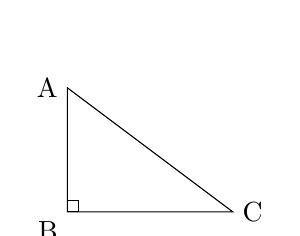
\begin{tikzpicture}[scale=0.35]
\draw (0,4.50) node[left]{A} -- (0,0) node[below left]{B} -- (6.00,0) node[right]{C} -- cycle;
\draw (0,0) rectangle (0.4,0.4);
\end{tikzpicture}
\end{center}

Calculer la valeur exacte de $\ensuremath{\mathrm{A}}\ensuremath{\mathrm{C}}$.

\medskip

\noindent\textbf{2.} Le triangle \ensuremath{\mathrm{D}}\ensuremath{\mathrm{E}}\ensuremath{\mathrm{F}} est rectangle en \ensuremath{\mathrm{E}}. On donne $\ensuremath{\mathrm{D}}\ensuremath{\mathrm{F}} = 75~\text{cm}$ et $\ensuremath{\mathrm{D}}\ensuremath{\mathrm{E}} = 21~\text{cm}$.

\begin{center}
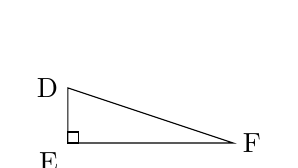
\begin{tikzpicture}[scale=0.35]
\draw (0,2.00) node[left]{D} -- (0,0) node[below left]{E} -- (6.00,0) node[right]{F} -- cycle;
\draw (0,0) rectangle (0.4,0.4);
\end{tikzpicture}
\end{center}

Calculer la valeur exacte de $\ensuremath{\mathrm{E}}\ensuremath{\mathrm{F}}$.

\medskip

\noindent\textbf{3.} Le triangle \ensuremath{\mathrm{M}}\ensuremath{\mathrm{N}}\ensuremath{\mathrm{P}} est rectangle en \ensuremath{\mathrm{N}}. On donne $\ensuremath{\mathrm{M}}\ensuremath{\mathrm{N}} = 7~\text{cm}$ et $\ensuremath{\mathrm{N}}\ensuremath{\mathrm{P}} = 12~\text{cm}$.

\begin{center}
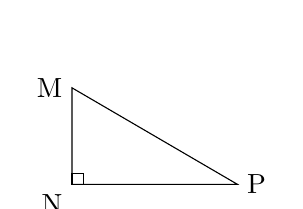
\begin{tikzpicture}[scale=0.35]
\draw (0,3.50) node[left]{M} -- (0,0) node[below left]{N} -- (6.00,0) node[right]{P} -- cycle;
\draw (0,0) rectangle (0.4,0.4);
\end{tikzpicture}
\end{center}

Calculer la valeur exacte de $\ensuremath{\mathrm{M}}\ensuremath{\mathrm{P}}$.

\medskip

\noindent\textbf{4.} Le triangle \ensuremath{\mathrm{R}}\ensuremath{\mathrm{S}}\ensuremath{\mathrm{T}} est rectangle en \ensuremath{\mathrm{S}}. On donne $\ensuremath{\mathrm{R}}\ensuremath{\mathrm{T}} = 11~\text{cm}$ et $\ensuremath{\mathrm{R}}\ensuremath{\mathrm{S}} = 3~\text{cm}$.

\begin{center}
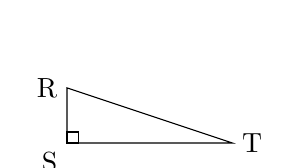
\begin{tikzpicture}[scale=0.35]
\draw (0,2.00) node[left]{R} -- (0,0) node[below left]{S} -- (6.00,0) node[right]{T} -- cycle;
\draw (0,0) rectangle (0.4,0.4);
\end{tikzpicture}
\end{center}

Calculer la valeur exacte de $\ensuremath{\mathrm{S}}\ensuremath{\mathrm{T}}$.

\medskip
\bigskip

\noindent\textbf{Exercice 7} -- Théorème de Thalès

\medskip
\noindent\textbf{1.} Les droites (\ensuremath{\mathrm{B}}\ensuremath{\mathrm{B}^\prime}) et (\ensuremath{\mathrm{C}}\ensuremath{\mathrm{C}^\prime}) sont parallèles. \ensuremath{\mathrm{A}}\ensuremath{\mathrm{B}^\prime} = 3, \ensuremath{\mathrm{A}}\ensuremath{\mathrm{C}} = 5, \ensuremath{\mathrm{A}}\ensuremath{\mathrm{B}} = 2.

\begin{center}
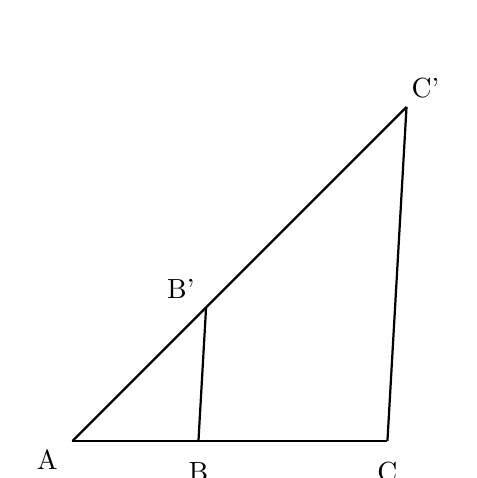
\begin{tikzpicture}[scale=0.8]
\draw [thick] (0.000,0.000)--(2.000,0.000);
\draw [thick] (2.000,0.000)--(5.000,0.000);
\draw [thick] (0.000,0.000)--(2.121,2.121);
\draw [thick] (2.121,2.121)--(5.303,5.303);
\draw [thick] (2.000,0.000)--(2.121,2.121);
\draw [thick] (5.000,0.000)--(5.303,5.303);
\draw (-0.400,-0.300) node {A};
\draw (2.000,-0.500) node {B};
\draw (5.000,-0.500) node {C};
\draw (1.721,2.421) node {B'};
\draw (5.603,5.603) node {C'};
\end{tikzpicture}
\end{center}
Déterminer en justifiant la valeur exacte de \ensuremath{\mathrm{A}}\ensuremath{\mathrm{C}^\prime}.

\bigskip
\noindent\textbf{2.} Les droites (\ensuremath{\mathrm{B}}\ensuremath{\mathrm{B}^\prime}) et (\ensuremath{\mathrm{C}}\ensuremath{\mathrm{C}^\prime}) sont parallèles. \ensuremath{\mathrm{A}}\ensuremath{\mathrm{B}^\prime} = 2, \ensuremath{\mathrm{A}}\ensuremath{\mathrm{B}} = 5, \ensuremath{\mathrm{A}}\ensuremath{\mathrm{C}} = 9.

\begin{center}
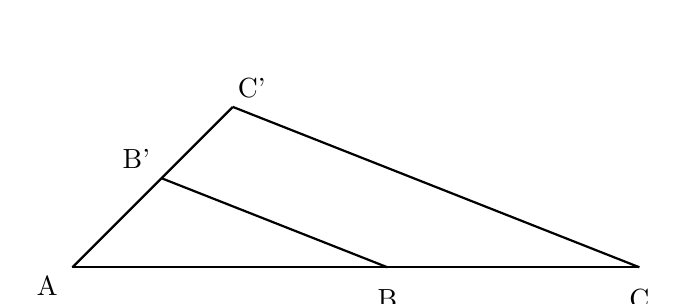
\begin{tikzpicture}[scale=0.8]
\draw [thick] (0.000,0.000)--(5.000,0.000);
\draw [thick] (5.000,0.000)--(9.000,0.000);
\draw [thick] (0.000,0.000)--(1.414,1.414);
\draw [thick] (1.414,1.414)--(2.546,2.546);
\draw [thick] (5.000,0.000)--(1.414,1.414);
\draw [thick] (9.000,0.000)--(2.546,2.546);
\draw (-0.400,-0.300) node {A};
\draw (5.000,-0.500) node {B};
\draw (9.000,-0.500) node {C};
\draw (1.014,1.714) node {B'};
\draw (2.846,2.846) node {C'};
\end{tikzpicture}
\end{center}
Déterminer en justifiant la valeur exacte de \ensuremath{\mathrm{A}}\ensuremath{\mathrm{C}^\prime}.

\bigskip
\noindent\textbf{3.} Les droites (\ensuremath{\mathrm{B}}\ensuremath{\mathrm{B}^\prime}) et (\ensuremath{\mathrm{C}}\ensuremath{\mathrm{C}^\prime}) sont parallèles. \ensuremath{\mathrm{A}}\ensuremath{\mathrm{B}} = 5, \ensuremath{\mathrm{A}}\ensuremath{\mathrm{C}} = 8, \ensuremath{\mathrm{A}}\ensuremath{\mathrm{B}^\prime} = 1.

\begin{center}
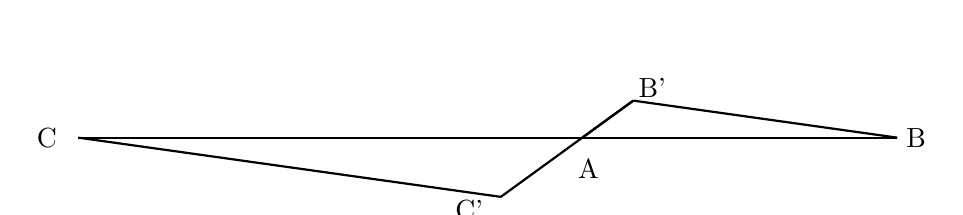
\begin{tikzpicture}[scale=0.8]
\draw [thick] (0.000,0.000)--(5.000,0.000);
\draw [thick] (5.000,0.000)--(-8.000,0.000);
\draw [thick] (0.000,0.000)--(0.809,0.588);
\draw [thick] (0.809,0.588)--(-1.294,-0.940);
\draw [thick] (5.000,0.000)--(0.809,0.588);
\draw [thick] (-8.000,0.000)--(-1.294,-0.940);
\draw (0.100,-0.500) node {A};
\draw (5.300,0.000) node {B};
\draw (-8.500,0.000) node {C};
\draw (1.109,0.788) node {B'};
\draw (-1.794,-1.140) node {C'};
\end{tikzpicture}
\end{center}
Déterminer en justifiant la valeur exacte de \ensuremath{\mathrm{A}}\ensuremath{\mathrm{C}^\prime}.

\bigskip
\noindent\textbf{4.} Les droites (\ensuremath{\mathrm{B}}\ensuremath{\mathrm{B}^\prime}) et (\ensuremath{\mathrm{C}}\ensuremath{\mathrm{C}^\prime}) sont parallèles. \ensuremath{\mathrm{A}}\ensuremath{\mathrm{B}^\prime} = 2, \ensuremath{\mathrm{A}}\ensuremath{\mathrm{B}} = 3, \ensuremath{\mathrm{A}}\ensuremath{\mathrm{C}} = 5.

\begin{center}
\begin{tikzpicture}[scale=0.8]
\draw [thick] (0.000,0.000)--(3.000,0.000);
\draw [thick] (3.000,0.000)--(-5.000,0.000);
\draw [thick] (0.000,0.000)--(1.618,1.176);
\draw [thick] (1.618,1.176)--(-2.697,-1.959);
\draw [thick] (3.000,0.000)--(1.618,1.176);
\draw [thick] (-5.000,0.000)--(-2.697,-1.959);
\draw (0.100,-0.500) node {A};
\draw (3.300,0.000) node {B};
\draw (-5.500,0.000) node {C};
\draw (1.918,1.376) node {B'};
\draw (-3.197,-2.159) node {C'};
\end{tikzpicture}
\end{center}
Déterminer en justifiant la valeur exacte de \ensuremath{\mathrm{A}}\ensuremath{\mathrm{C}^\prime}.
\bigskip

\noindent\textbf{Exercice 8} -- Résoudre les équations suivantes.
\begin{enumerate}
\item $7x = -10$
\item $13 - 8x = 13$
\item $-6x - 3 = 7$
\item $4x - 3 = 5x + 3$
\item $2x - 4 = -7x - 3$
\end{enumerate}
\bigskip

\noindent\textbf{Exercice 9} -- Résoudre les équations suivantes.
\begin{enumerate}
\item $(9 - 5x)(-3x - 9) = 0$
\item $(-7x - 7)(-5x - 8) = 0$
\item $(-5x - 6)(5x + 1) = 0$
\item $(-6x - 2)(5x - 2) = 0$
\end{enumerate}
\bigskip

\noindent\textbf{Exercice 10} -- Calculer et simplifier.
\begin{enumerate}
\item $\dfrac{3}{7} + \dfrac{4}{4}$
\item $\dfrac{2}{2} + \dfrac{10}{4}$
\item $\dfrac{3}{5} - \dfrac{3}{5} \times \dfrac{3}{5}$
\item $\dfrac{1}{5} - \dfrac{5}{6} \times \dfrac{5}{6}$
\item $\dfrac{5 + \dfrac{1}{2}}{\dfrac{3}{3} - \dfrac{3}{4}}$
\end{enumerate}
\bigskip

\noindent\textbf{Exercice 11} -- Factoriser les expressions suivantes.
\begin{enumerate}
\item $(6 - 6x)(3 - 6x) + (6 - 6x)(6x + 3)$
\item $(-6x - 6)(6 - 5x) + (-6x - 6)(2 - 5x)$
\item $(6x - 6)(7x - 7) + (6x - 6)(5x + 3)$
\end{enumerate}
\bigskip

\noindent\textbf{Exercice 12} -- Fonctions de référence.
\begin{enumerate}
\item $f(x) = \sqrt{x}. \text{ Comparer } f(2) \text{ et } f(9)$
\item $f(x) = x^3. \text{ Comparer } f(-5) \text{ et } f(2)$
\item $f(x) = \dfrac{1}{x}. \text{ Comparer } f(4) \text{ et } f(1)$
\item $f(x) = x^2. \text{ Résoudre } f(x) = 64$
\item $f(x) = x^2. \text{ Résoudre } f(x) = 25$
\end{enumerate}
\bigskip

\noindent\textbf{Exercice 13} -- Factoriser en utilisant une identité remarquable.
\begin{enumerate}
\item $(x - 8)^2 - 6^2$
\item $4x^2 + 32x + 64$
\item $(x - 6)^2 - 6^2$
\end{enumerate}
\bigskip

\noindent\textbf{Exercice 14} -- Intervalles et valeur absolue.
\begin{enumerate}
\item $\text{Le nombre } 1 \text{ appartient-il à } \left] -5 \,;\, 1 \right] \text{ ?}$
\item $\text{Le nombre } 4 \text{ appartient-il à } \left[ 3 \,;\, 5 \right[ \text{ ?}$
\item $|x + 8| < 2$
\item $|x - 3| < 1$
\item $|x - 3| \leqslant 2$
\end{enumerate}
\bigskip

\noindent\textbf{Exercice 15} -- Résoudre les inéquations suivantes.
\begin{enumerate}
\item $- 2 x > -2$
\item $- 3 x < 5$
\item $6 x - 5 \leq 3$
\item $2 x + 6 < -4$
\item $5 - 4 x > 2 x - 8$
\item $5 x + 6 \leq - 3 x - 3$
\end{enumerate}
\bigskip

\noindent\textbf{Exercice 16} -- Résoudre à l'aide d'un tableau de signes.
\begin{enumerate}
\item $\dfrac{4 x - 8}{- 5 x - 8} \leq 0$
\item $\dfrac{2 - x}{2 x + 4} > 0$
\item $\left(- 4 x - 4\right) \left(- 2 x - 1\right) < 0$
\item $\left(1 - 3 x\right) \left(9 - x\right) > 0$
\end{enumerate}
\bigskip

\noindent\textbf{Exercice 17} -- Écrire sous la forme d'une unique puissance de 10.
\begin{enumerate}
\item $\dfrac{10^{1} \times 10^{-3}}{10^{3}}$
\item $\dfrac{10^{0} \times (10^{1})^{3}}{10^{3}}$
\item $\dfrac{10^{-3} \times 10^{1}}{10^{1}}$
\item $\dfrac{10^{-2} \times (10^{2})^{2}}{10^{4}}$
\end{enumerate}
\bigskip

\noindent\textbf{Exercice 18} -- Calculer et simplifier.
\begin{enumerate}
\item $\sqrt{980}$
\item $\sqrt{28125}$
\item $2\sqrt{13} + 4\sqrt{2} + 4\sqrt{13} + 2\sqrt{2}$
\item $\sqrt{10} + 2\sqrt{5} + 4\sqrt{10} + 2\sqrt{5}$
\item $4\sqrt{50} - 2\sqrt{32} - 2\sqrt{72} + 3\sqrt{2}$
\item $(6 - 4\sqrt{11})^2$
\end{enumerate}
\bigskip

\noindent\textbf{Exercice 19} -- Vecteurs et coordonnées.\\
\medskip
\noindent\textbf{1)} Calculer les coordonnées de $\overrightarrow{\ensuremath{\mathrm{A}}\ensuremath{\mathrm{B}}}$.
\begin{enumerate}
\item $\ensuremath{\mathrm{A}}(0\,;\,5)$ et $\ensuremath{\mathrm{B}}(5\,;\,-4)$
\item $\ensuremath{\mathrm{A}}(-2\,;\,-2)$ et $\ensuremath{\mathrm{B}}(3\,;\,3)$
\item $\ensuremath{\mathrm{A}}(-3\,;\,-2)$ et $\ensuremath{\mathrm{B}}(-3\,;\,-3)$
\end{enumerate}
\medskip
\noindent\textbf{2)} Calculer les coordonnées du milieu de $[\ensuremath{\mathrm{A}}\ensuremath{\mathrm{B}}]$.
\begin{enumerate}
\item $\ensuremath{\mathrm{A}}(0\,;\,4)$ et $\ensuremath{\mathrm{B}}(-4\,;\,4)$
\item $\ensuremath{\mathrm{A}}(4\,;\,5)$ et $\ensuremath{\mathrm{B}}(8\,;\,-3)$
\end{enumerate}
\medskip
\noindent\textbf{3)} Les vecteurs $\vec{u}$ et $\vec{v}$ sont-ils colinéaires ?
\begin{enumerate}
\item $\vec{u}(5\,;\,-4)$ et $\vec{v}(4\,;\,-3)$
\item $\vec{u}(-4\,;\,3)$ et $\vec{v}(8\,;\,-6)$
\end{enumerate}
\bigskip

\noindent\textbf{Exercice 20} -- Équations de droites.
\medskip
\noindent\textbf{1)} Déterminer l'équation réduite de la droite $(\ensuremath{\mathrm{A}}\ensuremath{\mathrm{B}})$.
\begin{enumerate}
\item $\ensuremath{\mathrm{A}}(5\,;\,1)$ et $\ensuremath{\mathrm{B}}(1\,;\,-5)$
\item $\ensuremath{\mathrm{A}}(2\,;\,2)$ et $\ensuremath{\mathrm{B}}(-5\,;\,-2)$
\item $\ensuremath{\mathrm{A}}(-5\,;\,2)$ et $\ensuremath{\mathrm{B}}(-4\,;\,1)$
\end{enumerate}
\noindent\textbf{2)} Déterminer le point d'intersection.
\begin{enumerate}
\item $(d_1): y = -5x - 4$ et $(d_2): y = 2x + 3$
\item $(d_1): y = -3x - 3$ et $(d_2): y = 2x - 4$
\end{enumerate}
\bigskip

\vfill
\begin{flushright}
\qrset{height=1.5cm}
\qrset{level=M}
\qrcode{Ex1: 24x - 12 | 4x - 8 | -30x + 25 | -36x - 36 | 5(9x - 5) | 3(-4x - 5) | 6(3x + 7) | 2(-5x - 4)  //  Ex2: 37 | 45 | 54 | 24 | 71 | 66  //  Ex3: 9 | 7 | -8 | 23 | 3 | -39 | -31 | 18  //  Ex4: 28x^2 - 12x | -24x^2 + 18x | 36x^2 + 99x + 63 | -36x^2 - 78x - 36 | 14x^2 + 32x + 8 | -15x^2 + 51x - 18  //  Ex5: 12 - 14x | -16x - 3 | 15x - 1 | 3x + 7 | -13  //  Ex6: sqrt(100)~ cm | sqrt(5184)~ cm | sqrt(193)$ cm | sqrt(112)$ cm  //  Ex7: 15/2 | 18/5 | 8/5 | 10/3  //  Ex8: S = - (10)/(7) | S = 0 | S = - (5)/(3) | S = -6 | S = (1)/(9)  //  Ex9: S = -3 ; (9)/(5) | S = - (8)/(5) ; -1 | S = - (6)/(5) ; - (1)/(5) | S = - (1)/(3) ; (2)/(5)  //  Ex10: (10)/(7) | (7)/(2) | (6)/(25) | - (89)/(180) | 22  //  Ex11: (6 - 6x)(6) | (-6x - 6)(8 - 10x) | (6x - 6)(12x - 4)  //  Ex12: < | < | < | x = 8 ou x = -8 | x = 5 ou x = -5  //  Ex13: (x - 14)(x - 2) | (2x + 8)^2 | x(x - 12)  //  Ex14: Oui | Oui | ] -10 ; -6 [ | ] 2 ; 4 [ | [ 1 ; 5 ]  //  Ex15: ] -inf ; 1 [ | ] - (5)/(3) ; +inf [ | ] -inf ; (4)/(3) ] | ] -inf ; -5 [ | ] -inf ; (13)/(6) [ | ] -inf ; - (9)/(8) ]  //  Ex16: ] -inf ; - (8)/(5) [ U [ 2 ; +inf [ | ] -2 ; 2 [ | ] -1 ; - (1)/(2) [ | ] -inf ; (1)/(3) [ U ] 9 ; +inf [  //  Ex17: 10^-5 | 10^0 | 10^-3 | 10^-2  //  Ex18: 14 sqrt(5) | 75 sqrt(5) | 6 sqrt(2) + 6 sqrt(13) | 4 sqrt(5) + 5 sqrt(10) | 3 sqrt(2) | 212 - 48 sqrt(11)  //  Ex19: AB(5;-9) | AB(5;5) | AB(0;-1)  //  Ex20: y = (3)/(2)x - (13)/(2) | y = (4)/(7)x + (6)/(7) | y = -1x - 3}
\end{flushright}
\newpage
\begin{center}
\textbf{Corrigé numéro 1}\\
\end{center}

\noindent\textbf{Exercice 1}\par
\smallskip
\begin{enumerate}
\item $6(4x - 2) = 24x - 12$
\item $4(x - 2) = 4x - 8$
\item $5(-6x + 5) = -30x + 25$
\item $-9(4x + 4) = -36x - 36$
\end{enumerate}
\begin{enumerate}
\item $45x - 25 = 5(9x - 5)$
\item $-12x - 15 = 3(-4x - 5)$
\item $18x + 42 = 6(3x + 7)$
\item $-10x - 8 = 2(-5x - 4)$
\end{enumerate}
\medskip

\noindent\textbf{Exercice 2}\par
\smallskip
\begin{enumerate}
\item $2 \times (6 + 8) + 9$

$= 2 \times 14 + 9$

$= 28 + 9$

$= 37$
\item $(11 + 4) \times 3$

$= 15 \times 3$

$= 45$
\item $3 \times (8 + 7) + 9$

$= 3 \times 15 + 9$

$= 45 + 9$

$= 54$
\item $(10 + 2) \times 2$

$= 12 \times 2$

$= 24$
\item $6 \times (9 + 2) + 5$

$= 6 \times 11 + 5$

$= 66 + 5$

$= 71$
\item $(12 - 1) \times 6$

$= 11 \times 6$

$= 66$
\end{enumerate}
\medskip

\noindent\textbf{Exercice 3}\par
\smallskip
\begin{enumerate}
\item $(+19) + (+1) + (-11) = 9$
\item $(+11) + (+10) + (-14) = 7$
\item $(+5) + (-1) + (-12) = -8$
\item $(+14) + (-5) + (+14) = 23$
\item $(-10) + (-2) - (-15) = 3$
\item $(-11) - (+8) + (-20) = -39$
\item $(-20) - (+1) + (-10) = -31$
\item $(-4) - (-8) + (+14) = 18$
\end{enumerate}
\medskip

\noindent\textbf{Exercice 4}\par
\smallskip
\begin{enumerate}
\item $-4x(3 - 7x) = 28x^2 - 12x$
\item $6x(3 - 4x) = -24x^2 + 18x$
\item $(-9x - 9)(-4x - 7) = 36x^2 + 99x + 63$
\item $(-6x - 9)(6x + 4) = -36x^2 - 78x - 36$
\item $(2x + 4)(7x + 2) = 14x^2 + 32x + 8$
\item $(9 - 3x)(5x - 2) = -15x^2 + 51x - 18$
\end{enumerate}
\medskip

\noindent\textbf{Exercice 5}\par
\smallskip
\begin{enumerate}
\item $-(9x - 4)-(5x - 8) = 12 - 14x$
\item $-(9x + 9)+(6 - 7x) = -16x - 3$
\item $(9x + 6)-(7 - 6x) = 15x - 1$
\item $(8x + 4)+(3 - 5x) = 3x + 7$
\item $-(6x + 8)+(6x - 5) = -13$
\end{enumerate}
\medskip

\noindent\textbf{Exercice 6}\par
\smallskip
\textbf{1.} D'après le théorème de Pythagore dans le triangle \ensuremath{\mathrm{A}}\ensuremath{\mathrm{B}}\ensuremath{\mathrm{C}} rectangle en \ensuremath{\mathrm{B}} :

$\ensuremath{\mathrm{A}}\ensuremath{\mathrm{C}}^2 = \ensuremath{\mathrm{A}}\ensuremath{\mathrm{B}}^2 + \ensuremath{\mathrm{B}}\ensuremath{\mathrm{C}}^2$

$\ensuremath{\mathrm{A}}\ensuremath{\mathrm{C}}^2 = (6~\text{cm})^2 + (8~\text{cm})^2 = 36~\text{cm}^2 + 64~\text{cm}^2 = 100~\text{cm}^2$

Donc $\ensuremath{\mathrm{A}}\ensuremath{\mathrm{C}} = \sqrt{100}~\text{cm} = 10~\text{cm}$

\medskip
\textbf{2.} D'après le théorème de Pythagore dans le triangle \ensuremath{\mathrm{D}}\ensuremath{\mathrm{E}}\ensuremath{\mathrm{F}} rectangle en \ensuremath{\mathrm{E}} :

$\ensuremath{\mathrm{D}}\ensuremath{\mathrm{F}}^2 = \ensuremath{\mathrm{D}}\ensuremath{\mathrm{E}}^2 + \ensuremath{\mathrm{E}}\ensuremath{\mathrm{F}}^2$

Donc $\ensuremath{\mathrm{E}}\ensuremath{\mathrm{F}}^2 = \ensuremath{\mathrm{D}}\ensuremath{\mathrm{F}}^2 - \ensuremath{\mathrm{D}}\ensuremath{\mathrm{E}}^2 = (75~\text{cm})^2 - (21~\text{cm})^2 = 5625~\text{cm}^2 - 441~\text{cm}^2 = 5184~\text{cm}^2$

Donc $\ensuremath{\mathrm{E}}\ensuremath{\mathrm{F}} = \sqrt{5184}~\text{cm} = 72~\text{cm}$

\medskip
\textbf{3.} D'après le théorème de Pythagore :

$\ensuremath{\mathrm{M}}\ensuremath{\mathrm{P}}^2 = (7~\text{cm})^2 + (12~\text{cm})^2 = 49~\text{cm}^2 + 144~\text{cm}^2 = 193~\text{cm}^2$

Donc $\ensuremath{\mathrm{M}}\ensuremath{\mathrm{P}} = \sqrt{193}$ cm

\medskip
\textbf{4.} D'après le théorème de Pythagore :

$\ensuremath{\mathrm{R}}\ensuremath{\mathrm{T}}^2 = \ensuremath{\mathrm{R}}\ensuremath{\mathrm{S}}^2 + \ensuremath{\mathrm{S}}\ensuremath{\mathrm{T}}^2$

Donc $\ensuremath{\mathrm{S}}\ensuremath{\mathrm{T}}^2 = (11~\text{cm})^2 - (3~\text{cm})^2 = 121~\text{cm}^2 - 9~\text{cm}^2 = 112~\text{cm}^2$

Donc $\ensuremath{\mathrm{S}}\ensuremath{\mathrm{T}} = \sqrt{112}$ cm

\medskip
\medskip

\noindent\textbf{Exercice 7}\par
\smallskip
\textbf{1.} Comme (\ensuremath{\mathrm{B}}\ensuremath{\mathrm{B}^\prime}) et (\ensuremath{\mathrm{C}}\ensuremath{\mathrm{C}^\prime}) sont parallèles, d'après le théorème de Thalès : \[\dfrac{\ensuremath{\mathrm{A}}\ensuremath{\mathrm{C}^\prime}}{\ensuremath{\mathrm{A}}\ensuremath{\mathrm{C}}}=\dfrac{\ensuremath{\mathrm{A}}\ensuremath{\mathrm{B}^\prime}}{\ensuremath{\mathrm{A}}\ensuremath{\mathrm{B}}}=\dfrac{3}{2}.\]Donc \[\ensuremath{\mathrm{A}}\ensuremath{\mathrm{C}^\prime}=5\times\dfrac{3}{2}=\dfrac{15}{2}.\]\medskip
\textbf{2.} Comme (\ensuremath{\mathrm{B}}\ensuremath{\mathrm{B}^\prime}) et (\ensuremath{\mathrm{C}}\ensuremath{\mathrm{C}^\prime}) sont parallèles, d'après le théorème de Thalès : \[\dfrac{\ensuremath{\mathrm{A}}\ensuremath{\mathrm{C}^\prime}}{\ensuremath{\mathrm{A}}\ensuremath{\mathrm{C}}}=\dfrac{\ensuremath{\mathrm{A}}\ensuremath{\mathrm{B}^\prime}}{\ensuremath{\mathrm{A}}\ensuremath{\mathrm{B}}}=\dfrac{2}{5}.\]Donc \[\ensuremath{\mathrm{A}}\ensuremath{\mathrm{C}^\prime}=9\times\dfrac{2}{5}=\dfrac{18}{5}.\]\medskip
\textbf{3.} Comme (\ensuremath{\mathrm{B}}\ensuremath{\mathrm{B}^\prime}) et (\ensuremath{\mathrm{C}}\ensuremath{\mathrm{C}^\prime}) sont parallèles, d'après le théorème de Thalès : \[\dfrac{\ensuremath{\mathrm{A}}\ensuremath{\mathrm{C}^\prime}}{\ensuremath{\mathrm{A}}\ensuremath{\mathrm{C}}}=\dfrac{\ensuremath{\mathrm{A}}\ensuremath{\mathrm{B}^\prime}}{\ensuremath{\mathrm{A}}\ensuremath{\mathrm{B}}}=\dfrac{1}{5}.\]Donc \[\ensuremath{\mathrm{A}}\ensuremath{\mathrm{C}^\prime}=8\times\dfrac{1}{5}=\dfrac{8}{5}.\]\medskip
\textbf{4.} Comme (\ensuremath{\mathrm{B}}\ensuremath{\mathrm{B}^\prime}) et (\ensuremath{\mathrm{C}}\ensuremath{\mathrm{C}^\prime}) sont parallèles, d'après le théorème de Thalès : \[\dfrac{\ensuremath{\mathrm{A}}\ensuremath{\mathrm{C}^\prime}}{\ensuremath{\mathrm{A}}\ensuremath{\mathrm{C}}}=\dfrac{\ensuremath{\mathrm{A}}\ensuremath{\mathrm{B}^\prime}}{\ensuremath{\mathrm{A}}\ensuremath{\mathrm{B}}}=\dfrac{2}{3}.\]Donc \[\ensuremath{\mathrm{A}}\ensuremath{\mathrm{C}^\prime}=5\times\dfrac{2}{3}=\dfrac{10}{3}.\]\medskip
\medskip

\noindent\textbf{Exercice 8}\par
\smallskip
\begin{enumerate}
\item $7x = -10$

$\Leftrightarrow x = \dfrac{-10}{7} = - \dfrac{10}{7}$

L'ensemble des solutions est $S = \left\{- \dfrac{10}{7}\right\}$.

\item $13 - 8x = 13$

$\Leftrightarrow -8x = 13 - (13) = 0$

$\Leftrightarrow x = \dfrac{0}{-8} = 0$

L'ensemble des solutions est $S = \left\{0\right\}$.

\item $-6x - 3 = 7$

$\Leftrightarrow -6x = 7 - (-3) = 10$

$\Leftrightarrow x = \dfrac{10}{-6} = - \dfrac{5}{3}$

L'ensemble des solutions est $S = \left\{- \dfrac{5}{3}\right\}$.

\item $4x - 3 = 5x + 3$

$\Leftrightarrow -1x = 6$

$\Leftrightarrow x = \dfrac{6}{-1} = -6$

L'ensemble des solutions est $S = \left\{-6\right\}$.

\item $2x - 4 = -7x - 3$

$\Leftrightarrow 9x = 1$

$\Leftrightarrow x = \dfrac{1}{9} = \dfrac{1}{9}$

L'ensemble des solutions est $S = \left\{\dfrac{1}{9}\right\}$.

\end{enumerate}
\medskip

\noindent\textbf{Exercice 9}\par
\smallskip
\begin{enumerate}
\item Un produit est nul si et seulement si l'un des facteurs est nul.

$\bullet\ -3x - 9 = 0 \Leftrightarrow x = -3$

$\bullet\ 9 - 5x = 0 \Leftrightarrow x = \dfrac{9}{5}$

Donc $S = \left\{-3 \; ; \; \dfrac{9}{5}\right\}$

\item Un produit est nul si et seulement si l'un des facteurs est nul.

$\bullet\ -5x - 8 = 0 \Leftrightarrow x = - \dfrac{8}{5}$

$\bullet\ -7x - 7 = 0 \Leftrightarrow x = -1$

Donc $S = \left\{- \dfrac{8}{5} \; ; \; -1\right\}$

\item Un produit est nul si et seulement si l'un des facteurs est nul.

$\bullet\ -5x - 6 = 0 \Leftrightarrow x = - \dfrac{6}{5}$

$\bullet\ 5x + 1 = 0 \Leftrightarrow x = - \dfrac{1}{5}$

Donc $S = \left\{- \dfrac{6}{5} \; ; \; - \dfrac{1}{5}\right\}$

\item Un produit est nul si et seulement si l'un des facteurs est nul.

$\bullet\ -6x - 2 = 0 \Leftrightarrow x = - \dfrac{1}{3}$

$\bullet\ 5x - 2 = 0 \Leftrightarrow x = \dfrac{2}{5}$

Donc $S = \left\{- \dfrac{1}{3} \; ; \; \dfrac{2}{5}\right\}$

\end{enumerate}
\medskip

\noindent\textbf{Exercice 10}\par
\smallskip
\begin{enumerate}
\item $\dfrac{3 \times 4}{7 \times 4} + \dfrac{4 \times 7}{4 \times 7} = \dfrac{40}{28} = \dfrac{10}{7}$
\item $\dfrac{2 \times 2}{2 \times 2} + \dfrac{10 \times 1}{4 \times 1} = \dfrac{14}{4} = \dfrac{7}{2}$
\item $= \dfrac{3}{5} - \dfrac{9}{25}$ (priorité $\times$)

$= \dfrac{15}{25} - \dfrac{9}{25} = \dfrac{6}{25}$
\item $= \dfrac{1}{5} - \dfrac{25}{36}$ (priorité $\times$)

$= \dfrac{36}{180} - \dfrac{125}{180} = \dfrac{-89}{180}$
\item Numérateur : $5 + \dfrac{1}{2} = \dfrac{5 \times 2 + 1}{2} = \dfrac{11}{2}$

Dénominateur : $\dfrac{3}{3} - \dfrac{3}{4} = \dfrac{3 \times 4 - 3 \times 3}{3 \times 4} = \dfrac{1}{4}$

$= \dfrac{11}{2} \div \dfrac{1}{4} = \dfrac{11}{2} \times 4 = 22$
\end{enumerate}
\medskip

\noindent\textbf{Exercice 11}\par
\smallskip
\begin{enumerate}
\item $(6 - 6x)(6)$
\item $(-6x - 6)(8 - 10x)$
\item $(6x - 6)(12x - 4)$
\end{enumerate}
\medskip

\noindent\textbf{Exercice 12}\par
\smallskip
\begin{enumerate}
\item $\sqrt{x}$ est croissante sur $[0;+\infty[$. Comme $2 < 9$, $f(2) < f(9)$
\item $f(-5) = -125$ et $f(2) = 8$ donc $f(-5) < f(2)$
\item $f(4) = \dfrac{1}{4}$ et $f(1) = 1$ donc $f(4) < f(1)$
\item $x^2 = 64 \Longleftrightarrow x = \sqrt{64} = 8$ ou $x = -\sqrt{64} = -8$
\item $x^2 = 25 \Longleftrightarrow x = \sqrt{25} = 5$ ou $x = -\sqrt{25} = -5$
\end{enumerate}
\medskip

\noindent\textbf{Exercice 13}\par
\smallskip
\begin{enumerate}
\item $(x - 14)(x - 2)$
\item $(2x + 8)^2$
\item $x(x - 12)$
\end{enumerate}
\medskip

\noindent\textbf{Exercice 14}\par
\smallskip
\begin{enumerate}
\item $1$ $\in$ $\left] -5 \,;\, 1 \right]$
\item $4$ $\in$ $\left[ 3 \,;\, 5 \right[$
\item $|x + 8| < 2$

si et seulement si $-8 - 2 < x < -8 + 2$

si et seulement si $x \in \left] -10 \,;\, -6 \right[$
\item $|x - 3| < 1$

si et seulement si $3 - 1 < x < 3 + 1$

si et seulement si $x \in \left] 2 \,;\, 4 \right[$
\item $|x - 3| \leqslant 2$

si et seulement si $3 - 2 \leq x \leq 3 + 2$

si et seulement si $x \in \left[ 1 \,;\, 5 \right]$
\end{enumerate}
\medskip

\noindent\textbf{Exercice 15}\par
\smallskip
\begin{enumerate}
\item $-2x > -2$

$\Leftrightarrow x < 1$

$S = \left] -\infty \,;\, 1 \right[$
\item $-3x < 5$

$\Leftrightarrow x > - \dfrac{5}{3}$

$S = \left] - \dfrac{5}{3} \,;\, +\infty \right[$
\item $6 x - 5 \leq 3$

$\Leftrightarrow 6x \leq 3 - (-5) = 8$

$\Leftrightarrow x \leq \dfrac{4}{3}$

$S = \left] -\infty \,;\, \dfrac{4}{3} \right]$
\item $2 x + 6 < -4$

$\Leftrightarrow 2x < -4 - (6) = -10$

$\Leftrightarrow x < -5$

$S = \left] -\infty \,;\, -5 \right[$
\item $5 - 4 x > 2 x - 8$

$\Leftrightarrow -6x > -13$

$\Leftrightarrow x < \dfrac{13}{6}$

$S = \left] -\infty \,;\, \dfrac{13}{6} \right[$
\item $5 x + 6 \leq - 3 x - 3$

$\Leftrightarrow 8x \leq -9$

$\Leftrightarrow x \leq - \dfrac{9}{8}$

$S = \left] -\infty \,;\, - \dfrac{9}{8} \right]$
\end{enumerate}
\medskip

\noindent\textbf{Exercice 16}\par
\smallskip
\noindent\textbf{1)}\par\smallskip
\begin{center}
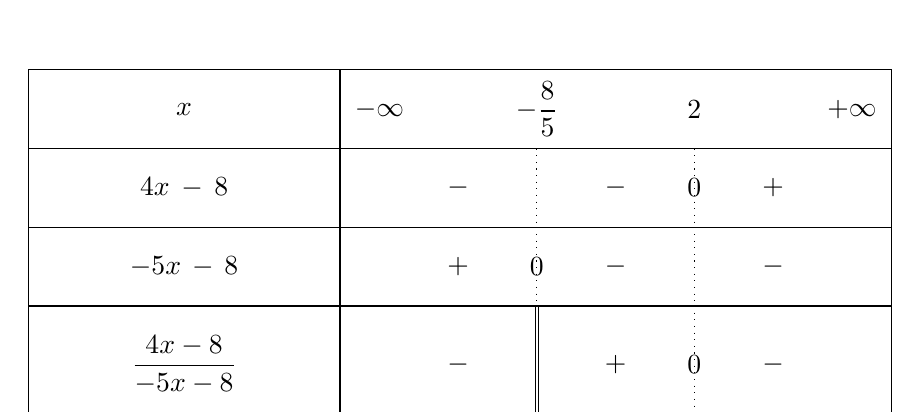
\begin{tikzpicture}
\tkzTabInit[lgt=3.96,espcl=2]{$x$ / 1, $4 x - 8$ / 1, $- 5 x - 8$ / 1, $\dfrac{4 x - 8}{- 5 x - 8}$ / 1.5}{$-\infty$, $- \dfrac{8}{5}$, $2$, $+\infty$}
\tkzTabLine{, -, t, -, z, +}
\tkzTabLine{, +, z, -, t, -}
\tkzTabLine{, -, d, +, z, -}
\end{tikzpicture}
\end{center}
\par\smallskip
\begin{center}$S = \left] -\infty \,;\, - \dfrac{8}{5} \right[ \cup \left[ 2 \,;\, +\infty \right[$\end{center}\par\medskip
\noindent\textbf{2)}\par\smallskip
\begin{center}
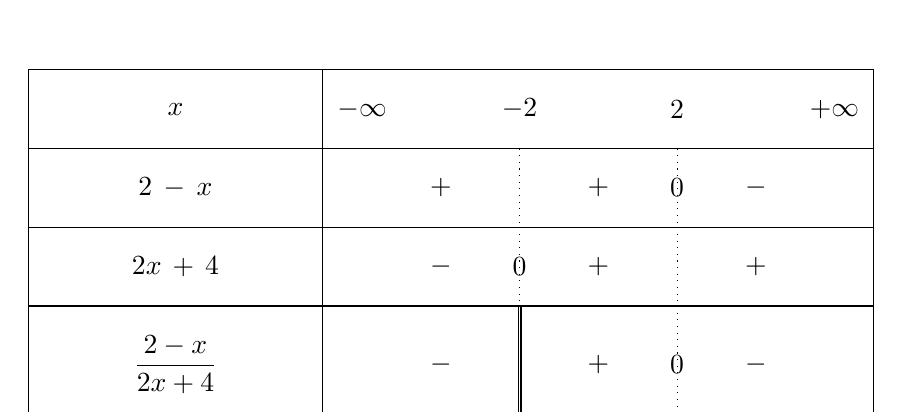
\begin{tikzpicture}
\tkzTabInit[lgt=3.74,espcl=2]{$x$ / 1, $2 - x$ / 1, $2 x + 4$ / 1, $\dfrac{2 - x}{2 x + 4}$ / 1.5}{$-\infty$, $-2$, $2$, $+\infty$}
\tkzTabLine{, +, t, +, z, -}
\tkzTabLine{, -, z, +, t, +}
\tkzTabLine{, -, d, +, z, -}
\end{tikzpicture}
\end{center}
\par\smallskip
\begin{center}$S = \left] -2 \,;\, 2 \right[$\end{center}\par\medskip
\noindent\textbf{3)}\par\smallskip
\begin{center}
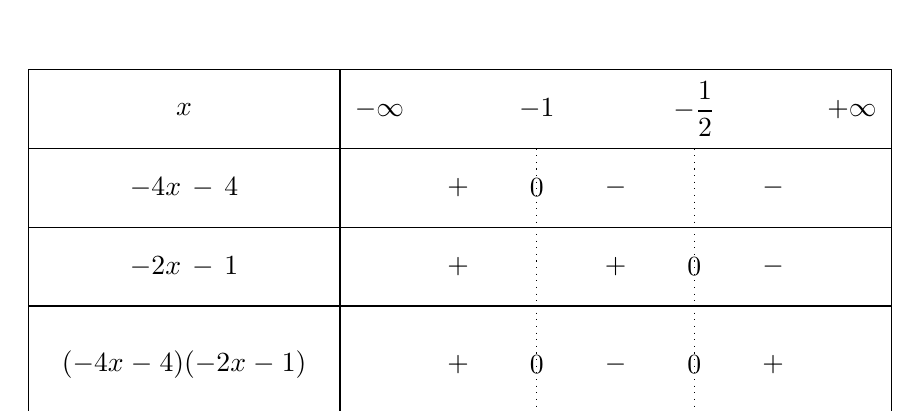
\begin{tikzpicture}
\tkzTabInit[lgt=3.96,espcl=2]{$x$ / 1, $- 4 x - 4$ / 1, $- 2 x - 1$ / 1, $(- 4 x - 4)(- 2 x - 1)$ / 1.5}{$-\infty$, $-1$, $- \dfrac{1}{2}$, $+\infty$}
\tkzTabLine{, +, z, -, t, -}
\tkzTabLine{, +, t, +, z, -}
\tkzTabLine{, +, z, -, z, +}
\end{tikzpicture}
\end{center}
\par\smallskip
\begin{center}$S = \left] -1 \,;\, - \dfrac{1}{2} \right[$\end{center}\par\medskip
\noindent\textbf{4)}\par\smallskip
\begin{center}
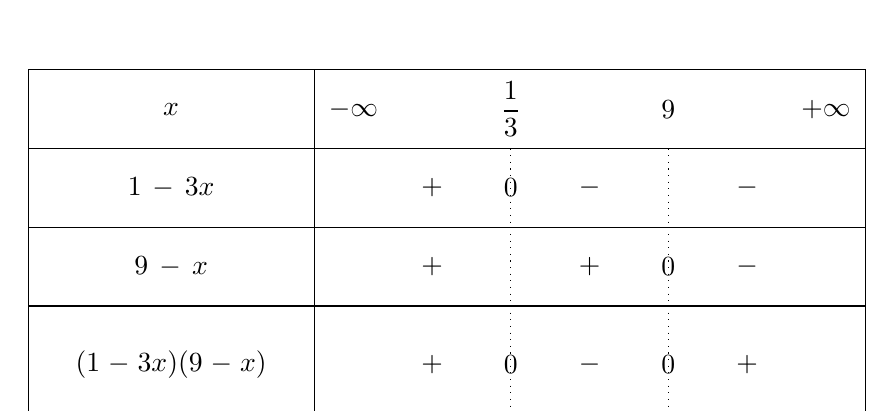
\begin{tikzpicture}
\tkzTabInit[lgt=3.63,espcl=2]{$x$ / 1, $1 - 3 x$ / 1, $9 - x$ / 1, $(1 - 3 x)(9 - x)$ / 1.5}{$-\infty$, $\dfrac{1}{3}$, $9$, $+\infty$}
\tkzTabLine{, +, z, -, t, -}
\tkzTabLine{, +, t, +, z, -}
\tkzTabLine{, +, z, -, z, +}
\end{tikzpicture}
\end{center}
\par\smallskip
\begin{center}$S = \left] -\infty \,;\, \dfrac{1}{3} \right[ \cup \left] 9 \,;\, +\infty \right[$\end{center}\par\medskip
\medskip

\noindent\textbf{Exercice 17}\par
\smallskip
\begin{enumerate}
\item $\dfrac{10^{1} \times 10^{-3}}{10^{3}} = 10^{-5}$
\item $\dfrac{10^{0} \times (10^{1})^{3}}{10^{3}} = 10^{0}$
\item $\dfrac{10^{-3} \times 10^{1}}{10^{1}} = 10^{-3}$
\item $\dfrac{10^{-2} \times (10^{2})^{2}}{10^{4}} = 10^{-2}$
\end{enumerate}
\medskip

\noindent\textbf{Exercice 18}\par
\smallskip
\begin{enumerate}
\item $14 \sqrt{5}$
\item $75 \sqrt{5}$
\item $6 \sqrt{2} + 6 \sqrt{13}$
\item $4 \sqrt{5} + 5 \sqrt{10}$
\item $3 \sqrt{2}$
\item $212 - 48 \sqrt{11}$
\end{enumerate}
\medskip

\noindent\textbf{Exercice 19}\par
\smallskip
\textbf{1)}
\begin{enumerate}
\item $\overrightarrow{\ensuremath{\mathrm{A}}\ensuremath{\mathrm{B}}}(5\,;\,-9)$
\item $\overrightarrow{\ensuremath{\mathrm{A}}\ensuremath{\mathrm{B}}}(5\,;\,5)$
\item $\overrightarrow{\ensuremath{\mathrm{A}}\ensuremath{\mathrm{B}}}(0\,;\,-1)$
\end{enumerate}
\textbf{2)}
\begin{enumerate}
\item $\ensuremath{\mathrm{M}}\left(-2\,;\,4\right)$
\item $\ensuremath{\mathrm{M}}\left(6\,;\,1\right)$
\end{enumerate}
\textbf{3)}
\begin{enumerate}
\item $\det(\vec{u},\vec{v}) = 5\times(-3)-(-4)\times4 = 1$. Non.
\item $\det(\vec{u},\vec{v}) = -4\times(-6)-(3)\times8 = 0$. Oui.
\end{enumerate}
\medskip

\noindent\textbf{Exercice 20}\par
\smallskip
\textbf{1)}
\begin{enumerate}
\item $m = \dfrac{-5-1}{1-5} = \dfrac{3}{2}$ donc $y = \dfrac{3}{2}x - \dfrac{13}{2}$
\item $m = \dfrac{-2-2}{-5-2} = \dfrac{4}{7}$ donc $y = \dfrac{4}{7}x + \dfrac{6}{7}$
\item $m = \dfrac{1-2}{-4--5} = -1$ donc $y = -1x - 3$
\end{enumerate}
\textbf{2)}
\begin{enumerate}
\item On cherche les couples $(x\,;\,y)$ vérifiant les deux équations :

$-5x - 4 = 2x + 3$

$\Leftrightarrow -7x = 7$

$\Leftrightarrow x = -1$

puis $y = -5 \times (-1) - 4 = 1$

Donc le point d'intersection est $\left(-1\,;\,1\right)$.
\item On cherche les couples $(x\,;\,y)$ vérifiant les deux équations :

$-3x - 3 = 2x - 4$

$\Leftrightarrow -5x = -1$

$\Leftrightarrow x = \dfrac{1}{5}$

puis $y = -3 \times (\dfrac{1}{5}) - 3 = - \dfrac{18}{5}$

Donc le point d'intersection est $\left(\dfrac{1}{5}\,;\,- \dfrac{18}{5}\right)$.
\end{enumerate}
\medskip

\newpage
\begin{center}
\textbf{Sujet numéro 2}
\\(à rendre avec la copie)
\end{center}


\noindent\textbf{Exercice 1} -- Développer les expressions suivantes.
\begin{enumerate}
\item $-5(-3x + 9)$
\item $2(-5x - 3)$
\item $7(-6x + 5)$
\item $6(x - 9)$
\end{enumerate}
\noindent\textbf{Exercice} -- Factoriser les expressions suivantes.
\begin{enumerate}
\item $-20x - 16$
\item $14x + 28$
\item $25x + 35$
\item $63x - 18$
\end{enumerate}
\bigskip

\noindent\textbf{Exercice 2} -- Calculer en respectant les priorités opératoires.
\begin{enumerate}
\item $(4 - 7) \times 5$
\item $5 \times (1 + 8) + 9$
\item $2 \times (10 - 1) + 2$
\item $3 \times (5 - 5) + 2$
\item $3 \times (1 + 8) - 4$
\item $2 \times (1 - 8) - 7$
\end{enumerate}
\bigskip

\noindent\textbf{Exercice 3} -- Calculer les expressions suivantes.
\begin{enumerate}
\item $(-4) + (+16) + (+11)$
\item $(+15) + (-7) + (-15)$
\item $(-13) + (-9) + (-8)$
\item $(-7) + (-14) + (+20)$
\item $(+1) + (-8) + (-1)$
\item $(-8) + (-16) + (-14)$
\item $(+10) + (+9) - (+7)$
\item $(0) + (-11) + (+7)$
\end{enumerate}
\bigskip

\noindent\textbf{Exercice 4} -- Développer et réduire.
\begin{enumerate}
\item $4x(8 - 9x)$
\item $-5x(-3x - 9)$
\item $(-4x - 5)(3x + 6)$
\item $(4 - 2x)(-6x - 4)$
\item $(-7x - 8)(9x + 2)$
\item $(-9x - 2)(-7x - 5)$
\end{enumerate}
\bigskip

\noindent\textbf{Exercice 5} -- Réduire les expressions suivantes.
\begin{enumerate}
\item $-(9x + 2)-(7x + 9)$
\item $(2x + 8)-(2 - 3x)$
\item $-(3 - 7x)-(4 - 8x)$
\item $(8 - 6x)+(-8x - 9)$
\item $-(3x + 6)+(-4x - 8)$
\end{enumerate}
\bigskip

\noindent\textbf{Exercice 6} -- Théorème de Pythagore.
\medskip

\noindent\textbf{1.} Le triangle \ensuremath{\mathrm{A}}\ensuremath{\mathrm{B}}\ensuremath{\mathrm{C}} est rectangle en \ensuremath{\mathrm{B}}. On donne $\ensuremath{\mathrm{A}}\ensuremath{\mathrm{B}} = 6~\text{cm}$ et $\ensuremath{\mathrm{B}}\ensuremath{\mathrm{C}} = 8~\text{cm}$.

\begin{center}
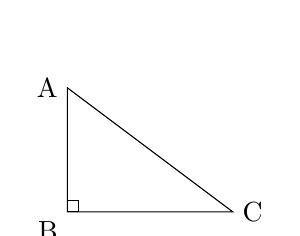
\begin{tikzpicture}[scale=0.35]
\draw (0,4.50) node[left]{A} -- (0,0) node[below left]{B} -- (6.00,0) node[right]{C} -- cycle;
\draw (0,0) rectangle (0.4,0.4);
\end{tikzpicture}
\end{center}

Calculer la valeur exacte de $\ensuremath{\mathrm{A}}\ensuremath{\mathrm{C}}$.

\medskip

\noindent\textbf{2.} Le triangle \ensuremath{\mathrm{D}}\ensuremath{\mathrm{E}}\ensuremath{\mathrm{F}} est rectangle en \ensuremath{\mathrm{E}}. On donne $\ensuremath{\mathrm{D}}\ensuremath{\mathrm{F}} = 15~\text{cm}$ et $\ensuremath{\mathrm{D}}\ensuremath{\mathrm{E}} = 9~\text{cm}$.

\begin{center}
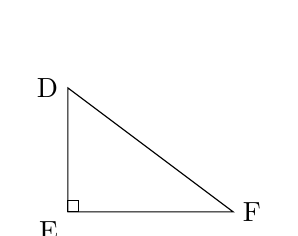
\begin{tikzpicture}[scale=0.35]
\draw (0,4.50) node[left]{D} -- (0,0) node[below left]{E} -- (6.00,0) node[right]{F} -- cycle;
\draw (0,0) rectangle (0.4,0.4);
\end{tikzpicture}
\end{center}

Calculer la valeur exacte de $\ensuremath{\mathrm{E}}\ensuremath{\mathrm{F}}$.

\medskip

\noindent\textbf{3.} Le triangle \ensuremath{\mathrm{M}}\ensuremath{\mathrm{N}}\ensuremath{\mathrm{P}} est rectangle en \ensuremath{\mathrm{N}}. On donne $\ensuremath{\mathrm{M}}\ensuremath{\mathrm{N}} = 5~\text{cm}$ et $\ensuremath{\mathrm{N}}\ensuremath{\mathrm{P}} = 9~\text{cm}$.

\begin{center}
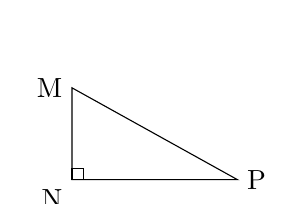
\begin{tikzpicture}[scale=0.35]
\draw (0,3.33) node[left]{M} -- (0,0) node[below left]{N} -- (6.00,0) node[right]{P} -- cycle;
\draw (0,0) rectangle (0.4,0.4);
\end{tikzpicture}
\end{center}

Calculer la valeur exacte de $\ensuremath{\mathrm{M}}\ensuremath{\mathrm{P}}$.

\medskip

\noindent\textbf{4.} Le triangle \ensuremath{\mathrm{R}}\ensuremath{\mathrm{S}}\ensuremath{\mathrm{T}} est rectangle en \ensuremath{\mathrm{S}}. On donne $\ensuremath{\mathrm{R}}\ensuremath{\mathrm{T}} = 8~\text{cm}$ et $\ensuremath{\mathrm{R}}\ensuremath{\mathrm{S}} = 2~\text{cm}$.

\begin{center}
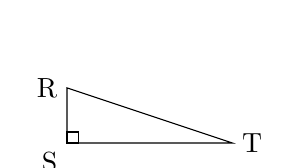
\begin{tikzpicture}[scale=0.35]
\draw (0,2.00) node[left]{R} -- (0,0) node[below left]{S} -- (6.00,0) node[right]{T} -- cycle;
\draw (0,0) rectangle (0.4,0.4);
\end{tikzpicture}
\end{center}

Calculer la valeur exacte de $\ensuremath{\mathrm{S}}\ensuremath{\mathrm{T}}$.

\medskip
\bigskip

\noindent\textbf{Exercice 7} -- Théorème de Thalès

\medskip
\noindent\textbf{1.} Les droites (\ensuremath{\mathrm{B}}\ensuremath{\mathrm{B}^\prime}) et (\ensuremath{\mathrm{C}}\ensuremath{\mathrm{C}^\prime}) sont parallèles. \ensuremath{\mathrm{A}}\ensuremath{\mathrm{B}} = 4, \ensuremath{\mathrm{A}}\ensuremath{\mathrm{C}} = 8, \ensuremath{\mathrm{A}}\ensuremath{\mathrm{B}^\prime} = 1.

\begin{center}
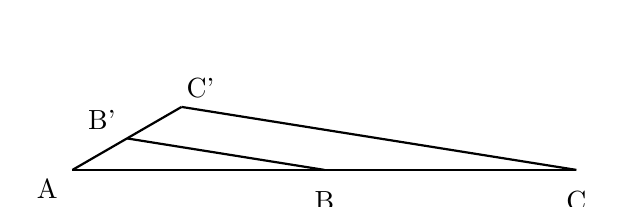
\begin{tikzpicture}[scale=0.8]
\draw [thick] (0.000,0.000)--(4.000,0.000);
\draw [thick] (4.000,0.000)--(8.000,0.000);
\draw [thick] (0.000,0.000)--(0.866,0.500);
\draw [thick] (0.866,0.500)--(1.732,1.000);
\draw [thick] (4.000,0.000)--(0.866,0.500);
\draw [thick] (8.000,0.000)--(1.732,1.000);
\draw (-0.400,-0.300) node {A};
\draw (4.000,-0.500) node {B};
\draw (8.000,-0.500) node {C};
\draw (0.466,0.800) node {B'};
\draw (2.032,1.300) node {C'};
\end{tikzpicture}
\end{center}
Déterminer en justifiant la valeur exacte de \ensuremath{\mathrm{A}}\ensuremath{\mathrm{C}^\prime}.

\bigskip
\noindent\textbf{2.} Les droites (\ensuremath{\mathrm{B}}\ensuremath{\mathrm{B}^\prime}) et (\ensuremath{\mathrm{C}}\ensuremath{\mathrm{C}^\prime}) sont parallèles. \ensuremath{\mathrm{A}}\ensuremath{\mathrm{C}} = 9, \ensuremath{\mathrm{A}}\ensuremath{\mathrm{B}^\prime} = 4, \ensuremath{\mathrm{A}}\ensuremath{\mathrm{B}} = 5.

\begin{center}
\begin{tikzpicture}[scale=0.8]
\draw [thick] (0.000,0.000)--(5.000,0.000);
\draw [thick] (5.000,0.000)--(9.000,0.000);
\draw [thick] (0.000,0.000)--(2.828,2.828);
\draw [thick] (2.828,2.828)--(5.091,5.091);
\draw [thick] (5.000,0.000)--(2.828,2.828);
\draw [thick] (9.000,0.000)--(5.091,5.091);
\draw (-0.400,-0.300) node {A};
\draw (5.000,-0.500) node {B};
\draw (9.000,-0.500) node {C};
\draw (2.428,3.128) node {B'};
\draw (5.391,5.391) node {C'};
\end{tikzpicture}
\end{center}
Déterminer en justifiant la valeur exacte de \ensuremath{\mathrm{A}}\ensuremath{\mathrm{C}^\prime}.

\bigskip
\noindent\textbf{3.} Les droites (\ensuremath{\mathrm{B}}\ensuremath{\mathrm{B}^\prime}) et (\ensuremath{\mathrm{C}}\ensuremath{\mathrm{C}^\prime}) sont parallèles. \ensuremath{\mathrm{A}}\ensuremath{\mathrm{B}^\prime} = 4, \ensuremath{\mathrm{A}}\ensuremath{\mathrm{C}} = 6, \ensuremath{\mathrm{A}}\ensuremath{\mathrm{B}} = 2.

\begin{center}
\begin{tikzpicture}[scale=0.8]
\draw [thick] (0.000,0.000)--(2.000,0.000);
\draw [thick] (2.000,0.000)--(-6.000,0.000);
\draw [thick] (0.000,0.000)--(2.828,2.828);
\draw [thick] (2.828,2.828)--(-8.485,-8.485);
\draw [thick] (2.000,0.000)--(2.828,2.828);
\draw [thick] (-6.000,0.000)--(-8.485,-8.485);
\draw (0.100,-0.500) node {A};
\draw (2.300,0.000) node {B};
\draw (-6.500,0.000) node {C};
\draw (3.128,3.028) node {B'};
\draw (-8.985,-8.685) node {C'};
\end{tikzpicture}
\end{center}
Déterminer en justifiant la valeur exacte de \ensuremath{\mathrm{A}}\ensuremath{\mathrm{C}^\prime}.

\bigskip
\noindent\textbf{4.} Les droites (\ensuremath{\mathrm{B}}\ensuremath{\mathrm{B}^\prime}) et (\ensuremath{\mathrm{C}}\ensuremath{\mathrm{C}^\prime}) sont parallèles. \ensuremath{\mathrm{A}}\ensuremath{\mathrm{C}} = 8, \ensuremath{\mathrm{A}}\ensuremath{\mathrm{B}^\prime} = 3, \ensuremath{\mathrm{A}}\ensuremath{\mathrm{B}} = 4.

\begin{center}
\begin{tikzpicture}[scale=0.8]
\draw [thick] (0.000,0.000)--(4.000,0.000);
\draw [thick] (4.000,0.000)--(-8.000,0.000);
\draw [thick] (0.000,0.000)--(2.121,2.121);
\draw [thick] (2.121,2.121)--(-4.243,-4.243);
\draw [thick] (4.000,0.000)--(2.121,2.121);
\draw [thick] (-8.000,0.000)--(-4.243,-4.243);
\draw (0.100,-0.500) node {A};
\draw (4.300,0.000) node {B};
\draw (-8.500,0.000) node {C};
\draw (2.421,2.321) node {B'};
\draw (-4.743,-4.443) node {C'};
\end{tikzpicture}
\end{center}
Déterminer en justifiant la valeur exacte de \ensuremath{\mathrm{A}}\ensuremath{\mathrm{C}^\prime}.
\bigskip

\noindent\textbf{Exercice 8} -- Résoudre les équations suivantes.
\begin{enumerate}
\item $3x = 20$
\item $7x + 1 = -6$
\item $-2x - 8 = -6$
\item $-5x - 11 = 8 - 7x$
\item $5 - 6x = 5x - 3$
\end{enumerate}
\bigskip

\noindent\textbf{Exercice 9} -- Résoudre les équations suivantes.
\begin{enumerate}
\item $(2x + 8)(5x - 5) = 0$
\item $(3 - 3x)(-4x - 6) = 0$
\item $(4x - 8)(7x + 7) = 0$
\item $(3x + 3)(6x + 6) = 0$
\end{enumerate}
\bigskip

\noindent\textbf{Exercice 10} -- Calculer et simplifier.
\begin{enumerate}
\item $\dfrac{3}{4} + \dfrac{6}{5}$
\item $\dfrac{9}{7} + \dfrac{3}{2}$
\item $\dfrac{1}{2} - \dfrac{4}{2} \times \dfrac{1}{4}$
\item $\dfrac{1}{2} - \dfrac{1}{5} \times \dfrac{2}{5}$
\item $\dfrac{4 + \dfrac{1}{2}}{\dfrac{5}{2} - \dfrac{1}{4}}$
\end{enumerate}
\bigskip

\noindent\textbf{Exercice 11} -- Factoriser les expressions suivantes.
\begin{enumerate}
\item $(-x - 2)(-5x - 3) + (-x - 2)(7x - 1)$
\item $(6 - x)(2x - 2) - (6 - x)(-4x - 1)$
\item $(3x - 7)(7x - 4) + (3x - 7)(3x + 7)$
\end{enumerate}
\bigskip

\noindent\textbf{Exercice 12} -- Fonctions de référence.
\begin{enumerate}
\item $f(x) = \sqrt{x}. \text{ Comparer } f(5) \text{ et } f(10)$
\item $f(x) = x^2. \text{ Comparer } f(-6) \text{ et } f(-7)$
\item $f(x) = \sqrt{x}. \text{ Résoudre } f(x) = 7$
\item $f(x) = \dfrac{1}{x}. \text{ Résoudre } f(x) = 1$
\item $f(x) = \dfrac{1}{x}. \text{ Résoudre } f(x) = \dfrac{3}{4}$
\end{enumerate}
\bigskip

\noindent\textbf{Exercice 13} -- Factoriser en utilisant une identité remarquable.
\begin{enumerate}
\item $(x - 1)^2 - (2x + 4)^2$
\item $4x^2 + 16x + 16$
\item $(x + 7)^2 - 3^2$
\end{enumerate}
\bigskip

\noindent\textbf{Exercice 14} -- Intervalles et valeur absolue.
\begin{enumerate}
\item $\text{Le nombre } -7 \text{ appartient-il à } \left[ -8 \,;\, -7 \right[ \text{ ?}$
\item $\text{Le nombre } 9 \text{ appartient-il à } \left[ 6 \,;\, 9 \right[ \text{ ?}$
\item $|x + 3| < 5$
\item $|x + 6| < 3$
\item $|x + 3| \leqslant 4$
\end{enumerate}
\bigskip

\noindent\textbf{Exercice 15} -- Résoudre les inéquations suivantes.
\begin{enumerate}
\item $2 x < -6$
\item $3 x > 2$
\item $3 x - 9 \geq -2$
\item $2 x + 4 < 2$
\item $5 x - 4 < 8 x - 7$
\item $8 - 5 x \geq 3 x + 9$
\end{enumerate}
\bigskip

\noindent\textbf{Exercice 16} -- Résoudre à l'aide d'un tableau de signes.
\begin{enumerate}
\item $\left(- 5 x - 6\right) \left(- 2 x - 3\right) < 0$
\item $\left(- 2 x - 7\right) \left(2 x - 3\right) \geq 0$
\item $\dfrac{2 x + 3}{2 - 3 x} > 0$
\item $\left(- 2 x - 9\right) \left(2 x + 7\right) \geq 0$
\end{enumerate}
\bigskip

\noindent\textbf{Exercice 17} -- Écrire sous la forme d'une unique puissance de 10.
\begin{enumerate}
\item $\dfrac{10^{1} \times 10^{-2}}{10^{1}}$
\item $\dfrac{10^{-3} \times (10^{1})^{3}}{10^{2}}$
\item $\dfrac{10^{0} \times 10^{0}}{10^{3}}$
\item $\dfrac{10^{-1} \times (10^{1})^{3}}{10^{3}}$
\end{enumerate}
\bigskip

\noindent\textbf{Exercice 18} -- Calculer et simplifier.
\begin{enumerate}
\item $\sqrt{48}$
\item $\sqrt{7203}$
\item $2\sqrt{3} + 3\sqrt{11} + 4\sqrt{3} - 2\sqrt{11}$
\item $5\sqrt{7} - 3\sqrt{2} - 4\sqrt{7} - \sqrt{2}$
\item $-3\sqrt{180} - 3\sqrt{5} - 4\sqrt{80} + 2\sqrt{45}$
\item $(2 - \sqrt{7})^2$
\end{enumerate}
\bigskip

\noindent\textbf{Exercice 19} -- Vecteurs et coordonnées.\\
\medskip
\noindent\textbf{1)} Calculer les coordonnées de $\overrightarrow{\ensuremath{\mathrm{A}}\ensuremath{\mathrm{B}}}$.
\begin{enumerate}
\item $\ensuremath{\mathrm{A}}(1\,;\,0)$ et $\ensuremath{\mathrm{B}}(4\,;\,-2)$
\item $\ensuremath{\mathrm{A}}(-1\,;\,-5)$ et $\ensuremath{\mathrm{B}}(-1\,;\,-4)$
\item $\ensuremath{\mathrm{A}}(0\,;\,-2)$ et $\ensuremath{\mathrm{B}}(2\,;\,-5)$
\end{enumerate}
\medskip
\noindent\textbf{2)} Calculer les coordonnées du milieu de $[\ensuremath{\mathrm{A}}\ensuremath{\mathrm{B}}]$.
\begin{enumerate}
\item $\ensuremath{\mathrm{A}}(8\,;\,3)$ et $\ensuremath{\mathrm{B}}(4\,;\,-3)$
\item $\ensuremath{\mathrm{A}}(-4\,;\,2)$ et $\ensuremath{\mathrm{B}}(5\,;\,-4)$
\end{enumerate}
\medskip
\noindent\textbf{3)} Les vecteurs $\vec{u}$ et $\vec{v}$ sont-ils colinéaires ?
\begin{enumerate}
\item $\vec{u}(4\,;\,-5)$ et $\vec{v}(-4\,;\,5)$
\item $\vec{u}(0\,;\,-2)$ et $\vec{v}(-3\,;\,-5)$
\end{enumerate}
\bigskip

\noindent\textbf{Exercice 20} -- Équations de droites.
\medskip
\noindent\textbf{1)} Déterminer l'équation réduite de la droite $(\ensuremath{\mathrm{A}}\ensuremath{\mathrm{B}})$.
\begin{enumerate}
\item $\ensuremath{\mathrm{A}}(2\,;\,2)$ et $\ensuremath{\mathrm{B}}(1\,;\,5)$
\item $\ensuremath{\mathrm{A}}(-4\,;\,-2)$ et $\ensuremath{\mathrm{B}}(4\,;\,3)$
\item $\ensuremath{\mathrm{A}}(-1\,;\,1)$ et $\ensuremath{\mathrm{B}}(0\,;\,-3)$
\end{enumerate}
\noindent\textbf{2)} Déterminer le point d'intersection.
\begin{enumerate}
\item $(d_1): y = 4x - 2$ et $(d_2): y = -5x + 5$
\item $(d_1): y = x$ et $(d_2): y = 2x$
\end{enumerate}
\bigskip

\vfill
\begin{flushright}
\qrset{height=1.5cm}
\qrset{level=M}
\qrcode{Ex1: 15x - 45 | -10x - 6 | -42x + 35 | 6x - 54 | 4(-5x - 4) | 7(2x + 4) | 5(5x + 7) | 9(7x - 2)  //  Ex2: -15 | 54 | 20 | 2 | 23 | -21  //  Ex3: 23 | -7 | -30 | -1 | -8 | -38 | 12 | -4  //  Ex4: -36x^2 + 32x | 15x^2 + 45x | -12x^2 - 39x - 30 | 12x^2 - 16x - 16 | -63x^2 - 86x - 16 | 63x^2 + 59x + 10  //  Ex5: -16x - 11 | 5x + 6 | 15x - 7 | -14x - 1 | -7x - 14  //  Ex6: sqrt(100)~ cm | sqrt(144)~ cm | sqrt(106)$ cm | sqrt(60)$ cm  //  Ex7: 2 | 36/5 | 12 | 6  //  Ex8: S = (20)/(3) | S = -1 | S = -1 | S = (19)/(2) | S = (8)/(11)  //  Ex9: S = -4 ; 1 | S = - (3)/(2) ; 1 | S = -1 ; 2 | S = -1  //  Ex10: (39)/(20) | (39)/(14) | 0 | (21)/(50) | 2  //  Ex11: (-x - 2)(2x - 4) | (6 - x)(6x - 1) | (3x - 7)(10x + 3)  //  Ex12: < | < | x = 49 | x = 1 | x = (4)/(3)  //  Ex13: -3(x + 1)(x + 5) | (2x + 4)^2 | (x + 4)(x + 10)  //  Ex14: Non | Non | ] -8 ; 2 [ | ] -9 ; -3 [ | [ -7 ; 1 ]  //  Ex15: ] -inf ; -3 [ | ] (2)/(3) ; +inf [ | [ (7)/(3) ; +inf [ | ] -inf ; -1 [ | ] 1 ; +inf [ | ] -inf ; - (1)/(8) ]  //  Ex16: ] - (3)/(2) ; - (6)/(5) [ | [ - (7)/(2) ; (3)/(2) ] | ] - (3)/(2) ; (2)/(3) [ | [ - (9)/(2) ; - (7)/(2) ]  //  Ex17: 10^-2 | 10^-2 | 10^-3 | 10^-1  //  Ex18: 4 sqrt(3) | 49 sqrt(3) | sqrt(11) + 6 sqrt(3) | - 4 sqrt(2) + sqrt(7) | - 31 sqrt(5) | 11 - 4 sqrt(7)  //  Ex19: AB(3;-2) | AB(0;1) | AB(2;-3)  //  Ex20: y = -3x + 8 | y = (5)/(8)x + (1)/(2) | y = -4x - 3}
\end{flushright}
\newpage
\begin{center}
\textbf{Corrigé numéro 2}\\
\end{center}

\noindent\textbf{Exercice 1}\par
\smallskip
\begin{enumerate}
\item $-5(-3x + 9) = 15x - 45$
\item $2(-5x - 3) = -10x - 6$
\item $7(-6x + 5) = -42x + 35$
\item $6(x - 9) = 6x - 54$
\end{enumerate}
\begin{enumerate}
\item $-20x - 16 = 4(-5x - 4)$
\item $14x + 28 = 7(2x + 4)$
\item $25x + 35 = 5(5x + 7)$
\item $63x - 18 = 9(7x - 2)$
\end{enumerate}
\medskip

\noindent\textbf{Exercice 2}\par
\smallskip
\begin{enumerate}
\item $(4 - 7) \times 5$

$= -3 \times 5$

$= -15$
\item $5 \times (1 + 8) + 9$

$= 5 \times 9 + 9$

$= 45 + 9$

$= 54$
\item $2 \times (10 - 1) + 2$

$= 2 \times 9 + 2$

$= 18 + 2$

$= 20$
\item $3 \times (5 - 5) + 2$

$= 3 \times 0 + 2$

$= 0 + 2$

$= 2$
\item $3 \times (1 + 8) - 4$

$= 3 \times 9 - 4$

$= 27 - 4$

$= 23$
\item $2 \times (1 - 8) - 7$

$= 2 \times -7 - 7$

$= -14 - 7$

$= -21$
\end{enumerate}
\medskip

\noindent\textbf{Exercice 3}\par
\smallskip
\begin{enumerate}
\item $(-4) + (+16) + (+11) = 23$
\item $(+15) + (-7) + (-15) = -7$
\item $(-13) + (-9) + (-8) = -30$
\item $(-7) + (-14) + (+20) = -1$
\item $(+1) + (-8) + (-1) = -8$
\item $(-8) + (-16) + (-14) = -38$
\item $(+10) + (+9) - (+7) = 12$
\item $(0) + (-11) + (+7) = -4$
\end{enumerate}
\medskip

\noindent\textbf{Exercice 4}\par
\smallskip
\begin{enumerate}
\item $4x(8 - 9x) = -36x^2 + 32x$
\item $-5x(-3x - 9) = 15x^2 + 45x$
\item $(-4x - 5)(3x + 6) = -12x^2 - 39x - 30$
\item $(4 - 2x)(-6x - 4) = 12x^2 - 16x - 16$
\item $(-7x - 8)(9x + 2) = -63x^2 - 86x - 16$
\item $(-9x - 2)(-7x - 5) = 63x^2 + 59x + 10$
\end{enumerate}
\medskip

\noindent\textbf{Exercice 5}\par
\smallskip
\begin{enumerate}
\item $-(9x + 2)-(7x + 9) = -16x - 11$
\item $(2x + 8)-(2 - 3x) = 5x + 6$
\item $-(3 - 7x)-(4 - 8x) = 15x - 7$
\item $(8 - 6x)+(-8x - 9) = -14x - 1$
\item $-(3x + 6)+(-4x - 8) = -7x - 14$
\end{enumerate}
\medskip

\noindent\textbf{Exercice 6}\par
\smallskip
\textbf{1.} D'après le théorème de Pythagore dans le triangle \ensuremath{\mathrm{A}}\ensuremath{\mathrm{B}}\ensuremath{\mathrm{C}} rectangle en \ensuremath{\mathrm{B}} :

$\ensuremath{\mathrm{A}}\ensuremath{\mathrm{C}}^2 = \ensuremath{\mathrm{A}}\ensuremath{\mathrm{B}}^2 + \ensuremath{\mathrm{B}}\ensuremath{\mathrm{C}}^2$

$\ensuremath{\mathrm{A}}\ensuremath{\mathrm{C}}^2 = (6~\text{cm})^2 + (8~\text{cm})^2 = 36~\text{cm}^2 + 64~\text{cm}^2 = 100~\text{cm}^2$

Donc $\ensuremath{\mathrm{A}}\ensuremath{\mathrm{C}} = \sqrt{100}~\text{cm} = 10~\text{cm}$

\medskip
\textbf{2.} D'après le théorème de Pythagore dans le triangle \ensuremath{\mathrm{D}}\ensuremath{\mathrm{E}}\ensuremath{\mathrm{F}} rectangle en \ensuremath{\mathrm{E}} :

$\ensuremath{\mathrm{D}}\ensuremath{\mathrm{F}}^2 = \ensuremath{\mathrm{D}}\ensuremath{\mathrm{E}}^2 + \ensuremath{\mathrm{E}}\ensuremath{\mathrm{F}}^2$

Donc $\ensuremath{\mathrm{E}}\ensuremath{\mathrm{F}}^2 = \ensuremath{\mathrm{D}}\ensuremath{\mathrm{F}}^2 - \ensuremath{\mathrm{D}}\ensuremath{\mathrm{E}}^2 = (15~\text{cm})^2 - (9~\text{cm})^2 = 225~\text{cm}^2 - 81~\text{cm}^2 = 144~\text{cm}^2$

Donc $\ensuremath{\mathrm{E}}\ensuremath{\mathrm{F}} = \sqrt{144}~\text{cm} = 12~\text{cm}$

\medskip
\textbf{3.} D'après le théorème de Pythagore :

$\ensuremath{\mathrm{M}}\ensuremath{\mathrm{P}}^2 = (5~\text{cm})^2 + (9~\text{cm})^2 = 25~\text{cm}^2 + 81~\text{cm}^2 = 106~\text{cm}^2$

Donc $\ensuremath{\mathrm{M}}\ensuremath{\mathrm{P}} = \sqrt{106}$ cm

\medskip
\textbf{4.} D'après le théorème de Pythagore :

$\ensuremath{\mathrm{R}}\ensuremath{\mathrm{T}}^2 = \ensuremath{\mathrm{R}}\ensuremath{\mathrm{S}}^2 + \ensuremath{\mathrm{S}}\ensuremath{\mathrm{T}}^2$

Donc $\ensuremath{\mathrm{S}}\ensuremath{\mathrm{T}}^2 = (8~\text{cm})^2 - (2~\text{cm})^2 = 64~\text{cm}^2 - 4~\text{cm}^2 = 60~\text{cm}^2$

Donc $\ensuremath{\mathrm{S}}\ensuremath{\mathrm{T}} = \sqrt{60}$ cm

\medskip
\medskip

\noindent\textbf{Exercice 7}\par
\smallskip
\textbf{1.} Comme (\ensuremath{\mathrm{B}}\ensuremath{\mathrm{B}^\prime}) et (\ensuremath{\mathrm{C}}\ensuremath{\mathrm{C}^\prime}) sont parallèles, d'après le théorème de Thalès : \[\dfrac{\ensuremath{\mathrm{A}}\ensuremath{\mathrm{C}^\prime}}{\ensuremath{\mathrm{A}}\ensuremath{\mathrm{C}}}=\dfrac{\ensuremath{\mathrm{A}}\ensuremath{\mathrm{B}^\prime}}{\ensuremath{\mathrm{A}}\ensuremath{\mathrm{B}}}=\dfrac{1}{4}.\]Donc \[\ensuremath{\mathrm{A}}\ensuremath{\mathrm{C}^\prime}=8\times\dfrac{1}{4}=2.\]\medskip
\textbf{2.} Comme (\ensuremath{\mathrm{B}}\ensuremath{\mathrm{B}^\prime}) et (\ensuremath{\mathrm{C}}\ensuremath{\mathrm{C}^\prime}) sont parallèles, d'après le théorème de Thalès : \[\dfrac{\ensuremath{\mathrm{A}}\ensuremath{\mathrm{C}^\prime}}{\ensuremath{\mathrm{A}}\ensuremath{\mathrm{C}}}=\dfrac{\ensuremath{\mathrm{A}}\ensuremath{\mathrm{B}^\prime}}{\ensuremath{\mathrm{A}}\ensuremath{\mathrm{B}}}=\dfrac{4}{5}.\]Donc \[\ensuremath{\mathrm{A}}\ensuremath{\mathrm{C}^\prime}=9\times\dfrac{4}{5}=\dfrac{36}{5}.\]\medskip
\textbf{3.} Comme (\ensuremath{\mathrm{B}}\ensuremath{\mathrm{B}^\prime}) et (\ensuremath{\mathrm{C}}\ensuremath{\mathrm{C}^\prime}) sont parallèles, d'après le théorème de Thalès : \[\dfrac{\ensuremath{\mathrm{A}}\ensuremath{\mathrm{C}^\prime}}{\ensuremath{\mathrm{A}}\ensuremath{\mathrm{C}}}=\dfrac{\ensuremath{\mathrm{A}}\ensuremath{\mathrm{B}^\prime}}{\ensuremath{\mathrm{A}}\ensuremath{\mathrm{B}}}=\dfrac{4}{2}.\]Donc \[\ensuremath{\mathrm{A}}\ensuremath{\mathrm{C}^\prime}=6\times\dfrac{4}{2}=12.\]\medskip
\textbf{4.} Comme (\ensuremath{\mathrm{B}}\ensuremath{\mathrm{B}^\prime}) et (\ensuremath{\mathrm{C}}\ensuremath{\mathrm{C}^\prime}) sont parallèles, d'après le théorème de Thalès : \[\dfrac{\ensuremath{\mathrm{A}}\ensuremath{\mathrm{C}^\prime}}{\ensuremath{\mathrm{A}}\ensuremath{\mathrm{C}}}=\dfrac{\ensuremath{\mathrm{A}}\ensuremath{\mathrm{B}^\prime}}{\ensuremath{\mathrm{A}}\ensuremath{\mathrm{B}}}=\dfrac{3}{4}.\]Donc \[\ensuremath{\mathrm{A}}\ensuremath{\mathrm{C}^\prime}=8\times\dfrac{3}{4}=6.\]\medskip
\medskip

\noindent\textbf{Exercice 8}\par
\smallskip
\begin{enumerate}
\item $3x = 20$

$\Leftrightarrow x = \dfrac{20}{3} = \dfrac{20}{3}$

L'ensemble des solutions est $S = \left\{\dfrac{20}{3}\right\}$.

\item $7x + 1 = -6$

$\Leftrightarrow 7x = -6 - (1) = -7$

$\Leftrightarrow x = \dfrac{-7}{7} = -1$

L'ensemble des solutions est $S = \left\{-1\right\}$.

\item $-2x - 8 = -6$

$\Leftrightarrow -2x = -6 - (-8) = 2$

$\Leftrightarrow x = \dfrac{2}{-2} = -1$

L'ensemble des solutions est $S = \left\{-1\right\}$.

\item $-5x - 11 = 8 - 7x$

$\Leftrightarrow 2x = 19$

$\Leftrightarrow x = \dfrac{19}{2} = \dfrac{19}{2}$

L'ensemble des solutions est $S = \left\{\dfrac{19}{2}\right\}$.

\item $5 - 6x = 5x - 3$

$\Leftrightarrow -11x = -8$

$\Leftrightarrow x = \dfrac{-8}{-11} = \dfrac{8}{11}$

L'ensemble des solutions est $S = \left\{\dfrac{8}{11}\right\}$.

\end{enumerate}
\medskip

\noindent\textbf{Exercice 9}\par
\smallskip
\begin{enumerate}
\item Un produit est nul si et seulement si l'un des facteurs est nul.

$\bullet\ 2x + 8 = 0 \Leftrightarrow x = -4$

$\bullet\ 5x - 5 = 0 \Leftrightarrow x = 1$

Donc $S = \left\{-4 \; ; \; 1\right\}$

\item Un produit est nul si et seulement si l'un des facteurs est nul.

$\bullet\ 3 - 3x = 0 \Leftrightarrow x = 1$

$\bullet\ -4x - 6 = 0 \Leftrightarrow x = - \dfrac{3}{2}$

Donc $S = \left\{- \dfrac{3}{2} \; ; \; 1\right\}$

\item Un produit est nul si et seulement si l'un des facteurs est nul.

$\bullet\ 7x + 7 = 0 \Leftrightarrow x = -1$

$\bullet\ 4x - 8 = 0 \Leftrightarrow x = 2$

Donc $S = \left\{-1 \; ; \; 2\right\}$

\item Un produit est nul si et seulement si l'un des facteurs est nul.

$\bullet\ 3x + 3 = 0 \Leftrightarrow x = -1$

$\bullet\ 6x + 6 = 0 \Leftrightarrow x = -1$

Donc $S = \left\{-1\right\}$

\end{enumerate}
\medskip

\noindent\textbf{Exercice 10}\par
\smallskip
\begin{enumerate}
\item $\dfrac{3 \times 5}{4 \times 5} + \dfrac{6 \times 4}{5 \times 4} = \dfrac{39}{20}$
\item $\dfrac{9 \times 2}{7 \times 2} + \dfrac{3 \times 7}{2 \times 7} = \dfrac{39}{14}$
\item $= \dfrac{1}{2} - \dfrac{1}{2}$ (priorité $\times$)

$= \dfrac{1 - 1}{2} = 0$
\item $= \dfrac{1}{2} - \dfrac{2}{25}$ (priorité $\times$)

$= \dfrac{25}{50} - \dfrac{4}{50} = \dfrac{21}{50}$
\item Numérateur : $4 + \dfrac{1}{2} = \dfrac{4 \times 2 + 1}{2} = \dfrac{9}{2}$

Dénominateur : $\dfrac{5}{2} - \dfrac{1}{4} = \dfrac{5 \times 4 - 1 \times 2}{2 \times 4} = \dfrac{9}{4}$

$= \dfrac{9}{2} \div \dfrac{9}{4} = \dfrac{9}{2} \times \dfrac{4}{9} = 2$
\end{enumerate}
\medskip

\noindent\textbf{Exercice 11}\par
\smallskip
\begin{enumerate}
\item $(-x - 2)(2x - 4)$
\item $(6 - x)(6x - 1)$
\item $(3x - 7)(10x + 3)$
\end{enumerate}
\medskip

\noindent\textbf{Exercice 12}\par
\smallskip
\begin{enumerate}
\item $\sqrt{x}$ est croissante sur $[0;+\infty[$. Comme $5 < 10$, $f(5) < f(10)$
\item $f(-6) = 36$ et $f(-7) = 49$ donc $f(-6) < f(-7)$
\item $\sqrt{x} = 7 \Longleftrightarrow x = 7^2 = 49$ (avec $x \geq 0$)
\item $\dfrac{1}{x} = 1 \Longleftrightarrow x = 1$
\item $\dfrac{1}{x} = \dfrac{3}{4} \Longleftrightarrow x = \dfrac{4}{3}$
\end{enumerate}
\medskip

\noindent\textbf{Exercice 13}\par
\smallskip
\begin{enumerate}
\item $-3(x + 1)(x + 5)$
\item $(2x + 4)^2$
\item $(x + 4)(x + 10)$
\end{enumerate}
\medskip

\noindent\textbf{Exercice 14}\par
\smallskip
\begin{enumerate}
\item $-7$ $\notin$ $\left[ -8 \,;\, -7 \right[$
\item $9$ $\notin$ $\left[ 6 \,;\, 9 \right[$
\item $|x + 3| < 5$

si et seulement si $-3 - 5 < x < -3 + 5$

si et seulement si $x \in \left] -8 \,;\, 2 \right[$
\item $|x + 6| < 3$

si et seulement si $-6 - 3 < x < -6 + 3$

si et seulement si $x \in \left] -9 \,;\, -3 \right[$
\item $|x + 3| \leqslant 4$

si et seulement si $-3 - 4 \leq x \leq -3 + 4$

si et seulement si $x \in \left[ -7 \,;\, 1 \right]$
\end{enumerate}
\medskip

\noindent\textbf{Exercice 15}\par
\smallskip
\begin{enumerate}
\item $2x < -6$

$\Leftrightarrow x < -3$

$S = \left] -\infty \,;\, -3 \right[$
\item $3x > 2$

$\Leftrightarrow x > \dfrac{2}{3}$

$S = \left] \dfrac{2}{3} \,;\, +\infty \right[$
\item $3 x - 9 \geq -2$

$\Leftrightarrow 3x \geq -2 - (-9) = 7$

$\Leftrightarrow x \geq \dfrac{7}{3}$

$S = \left[ \dfrac{7}{3} \,;\, +\infty \right[$
\item $2 x + 4 < 2$

$\Leftrightarrow 2x < 2 - (4) = -2$

$\Leftrightarrow x < -1$

$S = \left] -\infty \,;\, -1 \right[$
\item $5 x - 4 < 8 x - 7$

$\Leftrightarrow -3x < -3$

$\Leftrightarrow x > 1$

$S = \left] 1 \,;\, +\infty \right[$
\item $8 - 5 x \geq 3 x + 9$

$\Leftrightarrow -8x \geq 1$

$\Leftrightarrow x \leq - \dfrac{1}{8}$

$S = \left] -\infty \,;\, - \dfrac{1}{8} \right]$
\end{enumerate}
\medskip

\noindent\textbf{Exercice 16}\par
\smallskip
\noindent\textbf{1)}\par\smallskip
\begin{center}
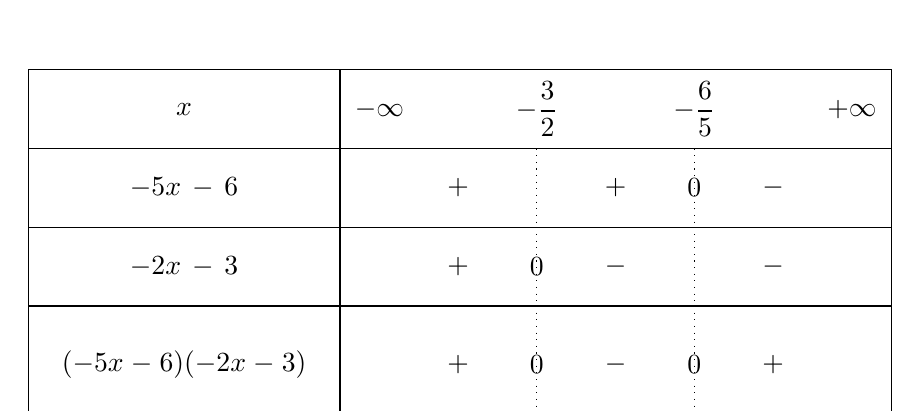
\begin{tikzpicture}
\tkzTabInit[lgt=3.96,espcl=2]{$x$ / 1, $- 5 x - 6$ / 1, $- 2 x - 3$ / 1, $(- 5 x - 6)(- 2 x - 3)$ / 1.5}{$-\infty$, $- \dfrac{3}{2}$, $- \dfrac{6}{5}$, $+\infty$}
\tkzTabLine{, +, t, +, z, -}
\tkzTabLine{, +, z, -, t, -}
\tkzTabLine{, +, z, -, z, +}
\end{tikzpicture}
\end{center}
\par\smallskip
\begin{center}$S = \left] - \dfrac{3}{2} \,;\, - \dfrac{6}{5} \right[$\end{center}\par\medskip
\noindent\textbf{2)}\par\smallskip
\begin{center}
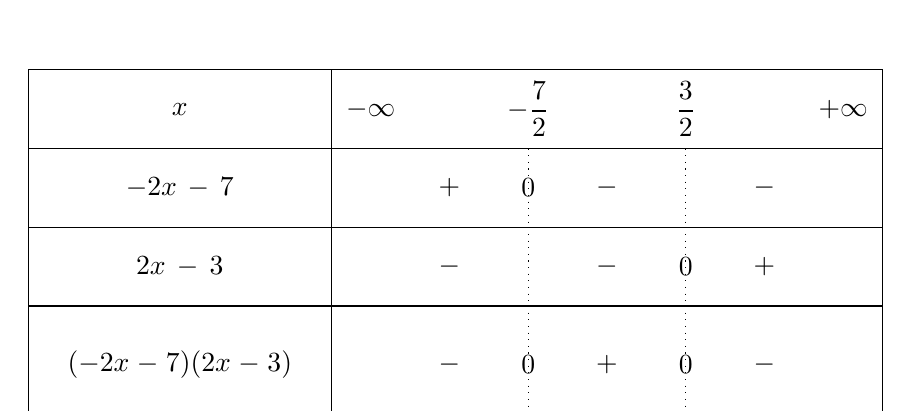
\begin{tikzpicture}
\tkzTabInit[lgt=3.85,espcl=2]{$x$ / 1, $- 2 x - 7$ / 1, $2 x - 3$ / 1, $(- 2 x - 7)(2 x - 3)$ / 1.5}{$-\infty$, $- \dfrac{7}{2}$, $\dfrac{3}{2}$, $+\infty$}
\tkzTabLine{, +, z, -, t, -}
\tkzTabLine{, -, t, -, z, +}
\tkzTabLine{, -, z, +, z, -}
\end{tikzpicture}
\end{center}
\par\smallskip
\begin{center}$S = \left[ - \dfrac{7}{2} \,;\, \dfrac{3}{2} \right]$\end{center}\par\medskip
\noindent\textbf{3)}\par\smallskip
\begin{center}
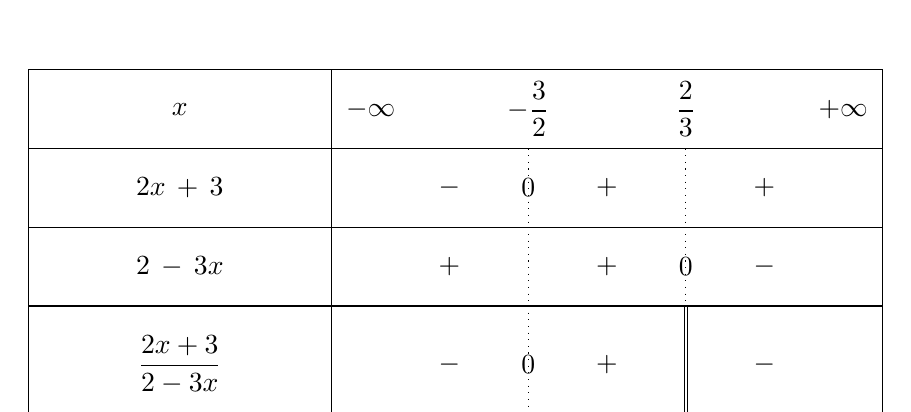
\begin{tikzpicture}
\tkzTabInit[lgt=3.85,espcl=2]{$x$ / 1, $2 x + 3$ / 1, $2 - 3 x$ / 1, $\dfrac{2 x + 3}{2 - 3 x}$ / 1.5}{$-\infty$, $- \dfrac{3}{2}$, $\dfrac{2}{3}$, $+\infty$}
\tkzTabLine{, -, z, +, t, +}
\tkzTabLine{, +, t, +, z, -}
\tkzTabLine{, -, z, +, d, -}
\end{tikzpicture}
\end{center}
\par\smallskip
\begin{center}$S = \left] - \dfrac{3}{2} \,;\, \dfrac{2}{3} \right[$\end{center}\par\medskip
\noindent\textbf{4)}\par\smallskip
\begin{center}
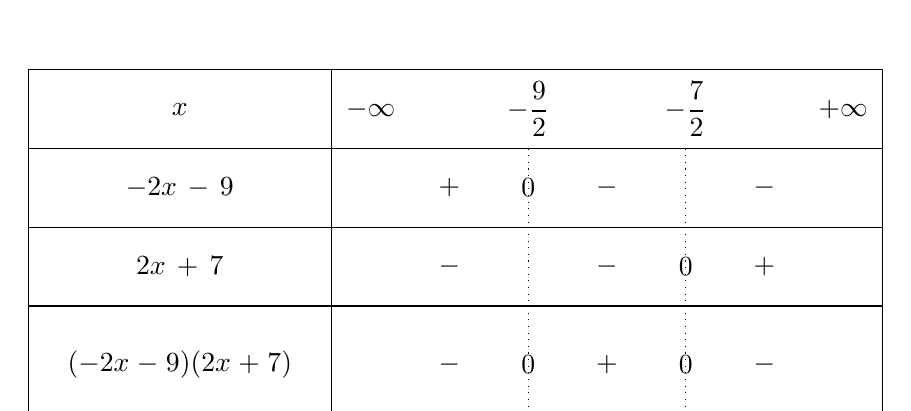
\begin{tikzpicture}
\tkzTabInit[lgt=3.85,espcl=2]{$x$ / 1, $- 2 x - 9$ / 1, $2 x + 7$ / 1, $(- 2 x - 9)(2 x + 7)$ / 1.5}{$-\infty$, $- \dfrac{9}{2}$, $- \dfrac{7}{2}$, $+\infty$}
\tkzTabLine{, +, z, -, t, -}
\tkzTabLine{, -, t, -, z, +}
\tkzTabLine{, -, z, +, z, -}
\end{tikzpicture}
\end{center}
\par\smallskip
\begin{center}$S = \left[ - \dfrac{9}{2} \,;\, - \dfrac{7}{2} \right]$\end{center}\par\medskip
\medskip

\noindent\textbf{Exercice 17}\par
\smallskip
\begin{enumerate}
\item $\dfrac{10^{1} \times 10^{-2}}{10^{1}} = 10^{-2}$
\item $\dfrac{10^{-3} \times (10^{1})^{3}}{10^{2}} = 10^{-2}$
\item $\dfrac{10^{0} \times 10^{0}}{10^{3}} = 10^{-3}$
\item $\dfrac{10^{-1} \times (10^{1})^{3}}{10^{3}} = 10^{-1}$
\end{enumerate}
\medskip

\noindent\textbf{Exercice 18}\par
\smallskip
\begin{enumerate}
\item $4 \sqrt{3}$
\item $49 \sqrt{3}$
\item $\sqrt{11} + 6 \sqrt{3}$
\item $- 4 \sqrt{2} + \sqrt{7}$
\item $- 31 \sqrt{5}$
\item $11 - 4 \sqrt{7}$
\end{enumerate}
\medskip

\noindent\textbf{Exercice 19}\par
\smallskip
\textbf{1)}
\begin{enumerate}
\item $\overrightarrow{\ensuremath{\mathrm{A}}\ensuremath{\mathrm{B}}}(3\,;\,-2)$
\item $\overrightarrow{\ensuremath{\mathrm{A}}\ensuremath{\mathrm{B}}}(0\,;\,1)$
\item $\overrightarrow{\ensuremath{\mathrm{A}}\ensuremath{\mathrm{B}}}(2\,;\,-3)$
\end{enumerate}
\textbf{2)}
\begin{enumerate}
\item $\ensuremath{\mathrm{M}}\left(6\,;\,0\right)$
\item $\ensuremath{\mathrm{M}}\left(\dfrac{1}{2}\,;\,-1\right)$
\end{enumerate}
\textbf{3)}
\begin{enumerate}
\item $\det(\vec{u},\vec{v}) = 4\times(5)-(-5)\times-4 = 0$. Oui.
\item $\det(\vec{u},\vec{v}) = 0\times(-5)-(-2)\times-3 = -6$. Non.
\end{enumerate}
\medskip

\noindent\textbf{Exercice 20}\par
\smallskip
\textbf{1)}
\begin{enumerate}
\item $m = \dfrac{5-2}{1-2} = -3$ donc $y = -3x + 8$
\item $m = \dfrac{3--2}{4--4} = \dfrac{5}{8}$ donc $y = \dfrac{5}{8}x + \dfrac{1}{2}$
\item $m = \dfrac{-3-1}{0--1} = -4$ donc $y = -4x - 3$
\end{enumerate}
\textbf{2)}
\begin{enumerate}
\item On cherche les couples $(x\,;\,y)$ vérifiant les deux équations :

$4x - 2 = -5x + 5$

$\Leftrightarrow 9x = 7$

$\Leftrightarrow x = \dfrac{7}{9}$

puis $y = 4 \times (\dfrac{7}{9}) - 2 = \dfrac{10}{9}$

Donc le point d'intersection est $\left(\dfrac{7}{9}\,;\,\dfrac{10}{9}\right)$.
\item On cherche les couples $(x\,;\,y)$ vérifiant les deux équations :

$x = 2x$

$\Leftrightarrow x = 0$

puis $y = 0 = 0$

Donc le point d'intersection est $\left(0\,;\,0\right)$.
\end{enumerate}
\medskip

\newpage
\begin{center}
\textbf{Sujet numéro 3}
\\(à rendre avec la copie)
\end{center}


\noindent\textbf{Exercice 1} -- Développer les expressions suivantes.
\begin{enumerate}
\item $4(x - 2)$
\item $-6(-9x - 8)$
\item $-9(-6x - 7)$
\item $3(x - 5)$
\end{enumerate}
\noindent\textbf{Exercice} -- Factoriser les expressions suivantes.
\begin{enumerate}
\item $40x + 25$
\item $-12x - 12$
\item $-35x - 30$
\item $40x - 35$
\end{enumerate}
\bigskip

\noindent\textbf{Exercice 2} -- Calculer en respectant les priorités opératoires.
\begin{enumerate}
\item $(13 - 1) \times 8$
\item $8 \times (5 + 1) + 6$
\item $4 \times (9 - 2) + 3$
\item $(3 - 8) \times 3$
\item $(5 + 6) \times 7$
\item $9 \times (9 + 4) - 4$
\end{enumerate}
\bigskip

\noindent\textbf{Exercice 3} -- Calculer les expressions suivantes.
\begin{enumerate}
\item $(-15) + (-1) + (-5)$
\item $(0) + (-18) + (+8)$
\item $(-11) + (-11) + (+2)$
\item $(-11) + (+20) + (-6)$
\item $(+13) - (+12) + (+20)$
\item $(+1) - (+9) - (+10)$
\item $(-15) - (+1) - (+14)$
\item $(-19) - (-20) + (-10)$
\end{enumerate}
\bigskip

\noindent\textbf{Exercice 4} -- Développer et réduire.
\begin{enumerate}
\item $9x(-8x - 7)$
\item $3x(7x + 2)$
\item $(5 - 8x)(-8x - 5)$
\item $(8 - 8x)(8 - 4x)$
\item $(-3x - 2)(3x + 7)$
\item $(-9x - 6)(6x - 6)$
\end{enumerate}
\bigskip

\noindent\textbf{Exercice 5} -- Réduire les expressions suivantes.
\begin{enumerate}
\item $-(4x + 3)-(3x + 6)$
\item $-(-8x - 4)+(-9x - 3)$
\item $(-4x - 3)+(-8x - 8)$
\item $(2 - 2x)+(3x - 6)$
\item $(-9x - 3)+(9x - 6)$
\end{enumerate}
\bigskip

\noindent\textbf{Exercice 6} -- Théorème de Pythagore.
\medskip

\noindent\textbf{1.} Le triangle \ensuremath{\mathrm{A}}\ensuremath{\mathrm{B}}\ensuremath{\mathrm{C}} est rectangle en \ensuremath{\mathrm{B}}. On donne $\ensuremath{\mathrm{A}}\ensuremath{\mathrm{B}} = 6~\text{cm}$ et $\ensuremath{\mathrm{B}}\ensuremath{\mathrm{C}} = 8~\text{cm}$.

\begin{center}
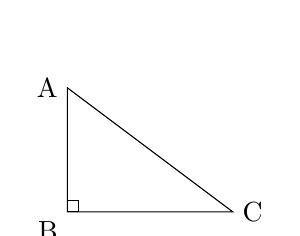
\begin{tikzpicture}[scale=0.35]
\draw (0,4.50) node[left]{A} -- (0,0) node[below left]{B} -- (6.00,0) node[right]{C} -- cycle;
\draw (0,0) rectangle (0.4,0.4);
\end{tikzpicture}
\end{center}

Calculer la valeur exacte de $\ensuremath{\mathrm{A}}\ensuremath{\mathrm{C}}$.

\medskip

\noindent\textbf{2.} Le triangle \ensuremath{\mathrm{D}}\ensuremath{\mathrm{E}}\ensuremath{\mathrm{F}} est rectangle en \ensuremath{\mathrm{E}}. On donne $\ensuremath{\mathrm{D}}\ensuremath{\mathrm{F}} = 75~\text{cm}$ et $\ensuremath{\mathrm{D}}\ensuremath{\mathrm{E}} = 21~\text{cm}$.

\begin{center}
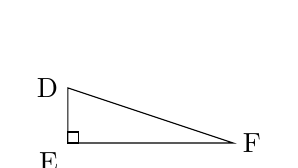
\begin{tikzpicture}[scale=0.35]
\draw (0,2.00) node[left]{D} -- (0,0) node[below left]{E} -- (6.00,0) node[right]{F} -- cycle;
\draw (0,0) rectangle (0.4,0.4);
\end{tikzpicture}
\end{center}

Calculer la valeur exacte de $\ensuremath{\mathrm{E}}\ensuremath{\mathrm{F}}$.

\medskip

\noindent\textbf{3.} Le triangle \ensuremath{\mathrm{M}}\ensuremath{\mathrm{N}}\ensuremath{\mathrm{P}} est rectangle en \ensuremath{\mathrm{N}}. On donne $\ensuremath{\mathrm{M}}\ensuremath{\mathrm{N}} = 8~\text{cm}$ et $\ensuremath{\mathrm{N}}\ensuremath{\mathrm{P}} = 10~\text{cm}$.

\begin{center}
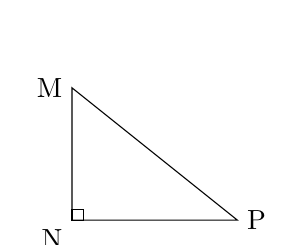
\begin{tikzpicture}[scale=0.35]
\draw (0,4.80) node[left]{M} -- (0,0) node[below left]{N} -- (6.00,0) node[right]{P} -- cycle;
\draw (0,0) rectangle (0.4,0.4);
\end{tikzpicture}
\end{center}

Calculer la valeur exacte de $\ensuremath{\mathrm{M}}\ensuremath{\mathrm{P}}$.

\medskip

\noindent\textbf{4.} Le triangle \ensuremath{\mathrm{R}}\ensuremath{\mathrm{S}}\ensuremath{\mathrm{T}} est rectangle en \ensuremath{\mathrm{S}}. On donne $\ensuremath{\mathrm{R}}\ensuremath{\mathrm{T}} = 5~\text{cm}$ et $\ensuremath{\mathrm{R}}\ensuremath{\mathrm{S}} = 3~\text{cm}$.

\begin{center}
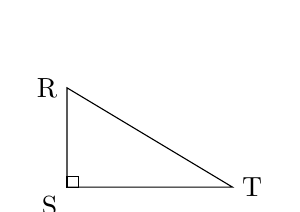
\begin{tikzpicture}[scale=0.35]
\draw (0,3.60) node[left]{R} -- (0,0) node[below left]{S} -- (6.00,0) node[right]{T} -- cycle;
\draw (0,0) rectangle (0.4,0.4);
\end{tikzpicture}
\end{center}

Calculer la valeur exacte de $\ensuremath{\mathrm{S}}\ensuremath{\mathrm{T}}$.

\medskip
\bigskip

\noindent\textbf{Exercice 7} -- Théorème de Thalès

\medskip
\noindent\textbf{1.} Les droites (\ensuremath{\mathrm{B}}\ensuremath{\mathrm{B}^\prime}) et (\ensuremath{\mathrm{C}}\ensuremath{\mathrm{C}^\prime}) sont parallèles. \ensuremath{\mathrm{A}}\ensuremath{\mathrm{C}} = 7, \ensuremath{\mathrm{A}}\ensuremath{\mathrm{B}^\prime} = 4, \ensuremath{\mathrm{A}}\ensuremath{\mathrm{B}} = 3.

\begin{center}
\begin{tikzpicture}[scale=0.8]
\draw [thick] (0.000,0.000)--(3.000,0.000);
\draw [thick] (3.000,0.000)--(7.000,0.000);
\draw [thick] (0.000,0.000)--(2.828,2.828);
\draw [thick] (2.828,2.828)--(6.600,6.600);
\draw [thick] (3.000,0.000)--(2.828,2.828);
\draw [thick] (7.000,0.000)--(6.600,6.600);
\draw (-0.400,-0.300) node {A};
\draw (3.000,-0.500) node {B};
\draw (7.000,-0.500) node {C};
\draw (2.428,3.128) node {B'};
\draw (6.900,6.900) node {C'};
\end{tikzpicture}
\end{center}
Déterminer en justifiant la valeur exacte de \ensuremath{\mathrm{A}}\ensuremath{\mathrm{C}^\prime}.

\bigskip
\noindent\textbf{2.} Les droites (\ensuremath{\mathrm{B}}\ensuremath{\mathrm{B}^\prime}) et (\ensuremath{\mathrm{C}}\ensuremath{\mathrm{C}^\prime}) sont parallèles. \ensuremath{\mathrm{A}}\ensuremath{\mathrm{B}} = 2, \ensuremath{\mathrm{A}}\ensuremath{\mathrm{C}} = 5, \ensuremath{\mathrm{A}}\ensuremath{\mathrm{B}^\prime} = 5.

\begin{center}
\begin{tikzpicture}[scale=0.8]
\draw [thick] (0.000,0.000)--(2.000,0.000);
\draw [thick] (2.000,0.000)--(5.000,0.000);
\draw [thick] (0.000,0.000)--(4.045,2.939);
\draw [thick] (4.045,2.939)--(10.113,7.347);
\draw [thick] (2.000,0.000)--(4.045,2.939);
\draw [thick] (5.000,0.000)--(10.113,7.347);
\draw (-0.400,-0.300) node {A};
\draw (2.000,-0.500) node {B};
\draw (5.000,-0.500) node {C};
\draw (3.645,3.239) node {B'};
\draw (10.413,7.647) node {C'};
\end{tikzpicture}
\end{center}
Déterminer en justifiant la valeur exacte de \ensuremath{\mathrm{A}}\ensuremath{\mathrm{C}^\prime}.

\bigskip
\noindent\textbf{3.} Les droites (\ensuremath{\mathrm{B}}\ensuremath{\mathrm{B}^\prime}) et (\ensuremath{\mathrm{C}}\ensuremath{\mathrm{C}^\prime}) sont parallèles. \ensuremath{\mathrm{A}}\ensuremath{\mathrm{B}^\prime} = 1, \ensuremath{\mathrm{A}}\ensuremath{\mathrm{C}} = 5, \ensuremath{\mathrm{A}}\ensuremath{\mathrm{B}} = 3.

\begin{center}
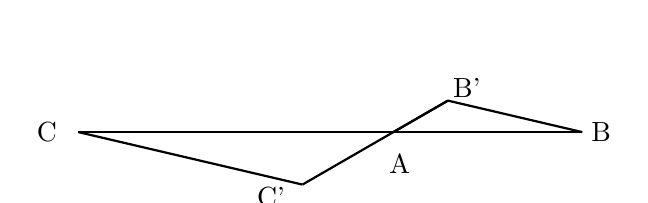
\begin{tikzpicture}[scale=0.8]
\draw [thick] (0.000,0.000)--(3.000,0.000);
\draw [thick] (3.000,0.000)--(-5.000,0.000);
\draw [thick] (0.000,0.000)--(0.866,0.500);
\draw [thick] (0.866,0.500)--(-1.443,-0.833);
\draw [thick] (3.000,0.000)--(0.866,0.500);
\draw [thick] (-5.000,0.000)--(-1.443,-0.833);
\draw (0.100,-0.500) node {A};
\draw (3.300,0.000) node {B};
\draw (-5.500,0.000) node {C};
\draw (1.166,0.700) node {B'};
\draw (-1.943,-1.033) node {C'};
\end{tikzpicture}
\end{center}
Déterminer en justifiant la valeur exacte de \ensuremath{\mathrm{A}}\ensuremath{\mathrm{C}^\prime}.

\bigskip
\noindent\textbf{4.} Les droites (\ensuremath{\mathrm{B}}\ensuremath{\mathrm{B}^\prime}) et (\ensuremath{\mathrm{C}}\ensuremath{\mathrm{C}^\prime}) sont parallèles. \ensuremath{\mathrm{A}}\ensuremath{\mathrm{B}^\prime} = 1, \ensuremath{\mathrm{A}}\ensuremath{\mathrm{C}} = 7, \ensuremath{\mathrm{A}}\ensuremath{\mathrm{B}} = 4.

\begin{center}
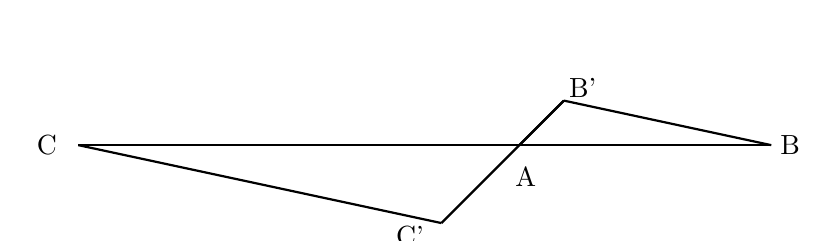
\begin{tikzpicture}[scale=0.8]
\draw [thick] (0.000,0.000)--(4.000,0.000);
\draw [thick] (4.000,0.000)--(-7.000,0.000);
\draw [thick] (0.000,0.000)--(0.707,0.707);
\draw [thick] (0.707,0.707)--(-1.237,-1.237);
\draw [thick] (4.000,0.000)--(0.707,0.707);
\draw [thick] (-7.000,0.000)--(-1.237,-1.237);
\draw (0.100,-0.500) node {A};
\draw (4.300,0.000) node {B};
\draw (-7.500,0.000) node {C};
\draw (1.007,0.907) node {B'};
\draw (-1.737,-1.437) node {C'};
\end{tikzpicture}
\end{center}
Déterminer en justifiant la valeur exacte de \ensuremath{\mathrm{A}}\ensuremath{\mathrm{C}^\prime}.
\bigskip

\noindent\textbf{Exercice 8} -- Résoudre les équations suivantes.
\begin{enumerate}
\item $-6x = 15$
\item $-7x - 6 = 11$
\item $8x + 7 = -8$
\item $7x - 10 = 4x - 6$
\item $-6x - 3 = -7x - 11$
\end{enumerate}
\bigskip

\noindent\textbf{Exercice 9} -- Résoudre les équations suivantes.
\begin{enumerate}
\item $(9 - 5x)(-5x - 7) = 0$
\item $(4x + 4)(6x + 2) = 0$
\item $(7 - 3x)(4x + 9) = 0$
\item $(x - 6)(x - 1) = 0$
\end{enumerate}
\bigskip

\noindent\textbf{Exercice 10} -- Calculer et simplifier.
\begin{enumerate}
\item $\dfrac{10}{7} - \dfrac{3}{5}$
\item $\dfrac{1}{10} + \dfrac{7}{3}$
\item $\dfrac{2}{2} - \dfrac{5}{4} \times \dfrac{4}{3}$
\item $\dfrac{5}{4} - \dfrac{1}{3} \times \dfrac{2}{3}$
\item $\dfrac{2 + \dfrac{2}{6}}{\dfrac{3}{6} - \dfrac{5}{4}}$
\end{enumerate}
\bigskip

\noindent\textbf{Exercice 11} -- Factoriser les expressions suivantes.
\begin{enumerate}
\item $(5x + 5)(6x - 3) + (5x + 5)(2 - 2x)$
\item $(6x + 3)(-6x - 2) + (6x + 3)(3x + 1)$
\item $(2x - 4)(7x - 7) + (2x - 4)(1 - 2x)$
\end{enumerate}
\bigskip

\noindent\textbf{Exercice 12} -- Fonctions de référence.
\begin{enumerate}
\item $f(x) = x^2. \text{ Comparer } f(5) \text{ et } f(-7)$
\item $f(x) = x^3. \text{ Comparer } f(-3) \text{ et } f(-1)$
\item $f(x) = x^3. \text{ Comparer } f(-3) \text{ et } f(2)$
\item $f(x) = x^2. \text{ Comparer } f(-7) \text{ et } f(2)$
\item $f(x) = \dfrac{1}{x}. \text{ Résoudre } f(x) = -1$
\end{enumerate}
\bigskip

\noindent\textbf{Exercice 13} -- Factoriser en utilisant une identité remarquable.
\begin{enumerate}
\item $(x - 4)^2 - 4^2$
\item $(x - 6)^2 - (4x + 1)^2$
\item $4x^2 + 8x + 4$
\end{enumerate}
\bigskip

\noindent\textbf{Exercice 14} -- Intervalles et valeur absolue.
\begin{enumerate}
\item $\text{Le nombre } -8 \text{ appartient-il à } \left] -7 \,;\, -3 \right[ \text{ ?}$
\item $\text{Le nombre } 4 \text{ appartient-il à } \left[ 4 \,;\, 9 \right] \text{ ?}$
\item $|x - 8| < 3$
\item $|x + 1| < 1$
\item $|x - 7| < 2$
\end{enumerate}
\bigskip

\noindent\textbf{Exercice 15} -- Résoudre les inéquations suivantes.
\begin{enumerate}
\item $2 x > -3$
\item $8 x < -5$
\item $9 - 3 x \leq 2$
\item $8 x + 6 \leq 3$
\item $8 x - 4 > 2 x + 3$
\item $4 x + 5 > 2 x - 6$
\end{enumerate}
\bigskip

\noindent\textbf{Exercice 16} -- Résoudre à l'aide d'un tableau de signes.
\begin{enumerate}
\item $\left(- 5 x - 5\right) \left(5 x + 3\right) \leq 0$
\item $\left(7 - 5 x\right) \left(- 3 x - 3\right) < 0$
\item $\left(- 5 x - 5\right) \left(2 x - 7\right) \leq 0$
\item $\left(- 3 x - 1\right) \left(x - 9\right) \leq 0$
\end{enumerate}
\bigskip

\noindent\textbf{Exercice 17} -- Écrire sous la forme d'une unique puissance de 10.
\begin{enumerate}
\item $\dfrac{10^{-3} \times 10^{3}}{10^{3}}$
\item $\dfrac{10^{-2} \times (10^{3})^{3}}{10^{4}}$
\item $\dfrac{10^{-2} \times 10^{0}}{10^{4}}$
\item $\dfrac{10^{-1} \times (10^{1})^{2}}{10^{4}}$
\end{enumerate}
\bigskip

\noindent\textbf{Exercice 18} -- Calculer et simplifier.
\begin{enumerate}
\item $\sqrt{8575}$
\item $\sqrt{12005}$
\item $3\sqrt{7} - \sqrt{2} - 3\sqrt{7} + 5\sqrt{2}$
\item $3\sqrt{13} + 2\sqrt{5} + 4\sqrt{13} - 5\sqrt{5}$
\item $-2\sqrt{5} - 2\sqrt{180} - 4\sqrt{20} - 4\sqrt{45}$
\item $(2 - 2\sqrt{3})^2$
\end{enumerate}
\bigskip

\noindent\textbf{Exercice 19} -- Vecteurs et coordonnées.\\
\medskip
\noindent\textbf{1)} Calculer les coordonnées de $\overrightarrow{\ensuremath{\mathrm{A}}\ensuremath{\mathrm{B}}}$.
\begin{enumerate}
\item $\ensuremath{\mathrm{A}}(3\,;\,4)$ et $\ensuremath{\mathrm{B}}(-4\,;\,0)$
\item $\ensuremath{\mathrm{A}}(0\,;\,0)$ et $\ensuremath{\mathrm{B}}(3\,;\,-3)$
\item $\ensuremath{\mathrm{A}}(4\,;\,3)$ et $\ensuremath{\mathrm{B}}(4\,;\,5)$
\end{enumerate}
\medskip
\noindent\textbf{2)} Calculer les coordonnées du milieu de $[\ensuremath{\mathrm{A}}\ensuremath{\mathrm{B}}]$.
\begin{enumerate}
\item $\ensuremath{\mathrm{A}}(-7\,;\,-7)$ et $\ensuremath{\mathrm{B}}(5\,;\,-7)$
\item $\ensuremath{\mathrm{A}}(-8\,;\,0)$ et $\ensuremath{\mathrm{B}}(6\,;\,2)$
\end{enumerate}
\medskip
\noindent\textbf{3)} Les vecteurs $\vec{u}$ et $\vec{v}$ sont-ils colinéaires ?
\begin{enumerate}
\item $\vec{u}(1\,;\,3)$ et $\vec{v}(2\,;\,6)$
\item $\vec{u}(-2\,;\,-2)$ et $\vec{v}(-5\,;\,-4)$
\end{enumerate}
\bigskip

\noindent\textbf{Exercice 20} -- Équations de droites.
\medskip
\noindent\textbf{1)} Déterminer l'équation réduite de la droite $(\ensuremath{\mathrm{A}}\ensuremath{\mathrm{B}})$.
\begin{enumerate}
\item $\ensuremath{\mathrm{A}}(-4\,;\,-5)$ et $\ensuremath{\mathrm{B}}(0\,;\,-2)$
\item $\ensuremath{\mathrm{A}}(3\,;\,4)$ et $\ensuremath{\mathrm{B}}(0\,;\,2)$
\item $\ensuremath{\mathrm{A}}(1\,;\,1)$ et $\ensuremath{\mathrm{B}}(4\,;\,2)$
\end{enumerate}
\noindent\textbf{2)} Déterminer le point d'intersection.
\begin{enumerate}
\item $(d_1): y = 5x + 3$ et $(d_2): y = -3x - 3$
\item $(d_1): y = -x - 5$ et $(d_2): y = 5x + 4$
\end{enumerate}
\bigskip

\vfill
\begin{flushright}
\qrset{height=1.5cm}
\qrset{level=M}
\qrcode{Ex1: 4x - 8 | 54x + 48 | 54x + 63 | 3x - 15 | 5(8x + 5) | 6(-2x - 2) | 5(-7x - 6) | 5(8x - 7)  //  Ex2: 96 | 54 | 31 | -15 | 77 | 113  //  Ex3: -21 | -10 | -20 | 3 | 21 | -18 | -30 | -9  //  Ex4: -72x^2 - 63x | 21x^2 + 6x | 64x^2 - 25 | 32x^2 - 96x + 64 | -9x^2 - 27x - 14 | -54x^2 + 18x + 36  //  Ex5: -7x - 9 | 1 - x | -12x - 11 | x - 4 | -9  //  Ex6: sqrt(100)~ cm | sqrt(5184)~ cm | sqrt(164)$ cm | sqrt(16)$ cm  //  Ex7: 28/3 | 25/2 | 5/3 | 7/4  //  Ex8: S = - (5)/(2) | S = - (17)/(7) | S = - (15)/(8) | S = (4)/(3) | S = -8  //  Ex9: S = - (7)/(5) ; (9)/(5) | S = -1 ; - (1)/(3) | S = - (9)/(4) ; (7)/(3) | S = 1 ; 6  //  Ex10: (29)/(35) | (73)/(30) | - (2)/(3) | (37)/(36) | - (28)/(9)  //  Ex11: (5x + 5)(4x - 1) | (6x + 3)(-3x - 1) | (2x - 4)(5x - 6)  //  Ex12: < | < | < | > | x = -1  //  Ex13: x(x - 8) | -5(x - 1)(3x + 7) | (2x + 2)^2  //  Ex14: Non | Oui | ] 5 ; 11 [ | ] -2 ; 0 [ | ] 5 ; 9 [  //  Ex15: ] - (3)/(2) ; +inf [ | ] -inf ; - (5)/(8) [ | [ (7)/(3) ; +inf [ | ] -inf ; - (3)/(8) ] | ] (7)/(6) ; +inf [ | ] - (11)/(2) ; +inf [  //  Ex16: ] -inf ; -1 ] U [ - (3)/(5) ; +inf [ | ] -1 ; (7)/(5) [ | ] -inf ; -1 ] U [ (7)/(2) ; +inf [ | ] -inf ; - (1)/(3) ] U [ 9 ; +inf [  //  Ex17: 10^-3 | 10^3 | 10^-6 | 10^-3  //  Ex18: 35 sqrt(7) | 49 sqrt(5) | 4 sqrt(2) | - 3 sqrt(5) + 7 sqrt(13) | - 34 sqrt(5) | 16 - 8 sqrt(3)  //  Ex19: AB(-7;-4) | AB(3;-3) | AB(0;2)  //  Ex20: y = (3)/(4)x - 2 | y = (2)/(3)x + 2 | y = (1)/(3)x + (2)/(3)}
\end{flushright}
\newpage
\begin{center}
\textbf{Corrigé numéro 3}\\
\end{center}

\noindent\textbf{Exercice 1}\par
\smallskip
\begin{enumerate}
\item $4(x - 2) = 4x - 8$
\item $-6(-9x - 8) = 54x + 48$
\item $-9(-6x - 7) = 54x + 63$
\item $3(x - 5) = 3x - 15$
\end{enumerate}
\begin{enumerate}
\item $40x + 25 = 5(8x + 5)$
\item $-12x - 12 = 6(-2x - 2)$
\item $-35x - 30 = 5(-7x - 6)$
\item $40x - 35 = 5(8x - 7)$
\end{enumerate}
\medskip

\noindent\textbf{Exercice 2}\par
\smallskip
\begin{enumerate}
\item $(13 - 1) \times 8$

$= 12 \times 8$

$= 96$
\item $8 \times (5 + 1) + 6$

$= 8 \times 6 + 6$

$= 48 + 6$

$= 54$
\item $4 \times (9 - 2) + 3$

$= 4 \times 7 + 3$

$= 28 + 3$

$= 31$
\item $(3 - 8) \times 3$

$= -5 \times 3$

$= -15$
\item $(5 + 6) \times 7$

$= 11 \times 7$

$= 77$
\item $9 \times (9 + 4) - 4$

$= 9 \times 13 - 4$

$= 117 - 4$

$= 113$
\end{enumerate}
\medskip

\noindent\textbf{Exercice 3}\par
\smallskip
\begin{enumerate}
\item $(-15) + (-1) + (-5) = -21$
\item $(0) + (-18) + (+8) = -10$
\item $(-11) + (-11) + (+2) = -20$
\item $(-11) + (+20) + (-6) = 3$
\item $(+13) - (+12) + (+20) = 21$
\item $(+1) - (+9) - (+10) = -18$
\item $(-15) - (+1) - (+14) = -30$
\item $(-19) - (-20) + (-10) = -9$
\end{enumerate}
\medskip

\noindent\textbf{Exercice 4}\par
\smallskip
\begin{enumerate}
\item $9x(-8x - 7) = -72x^2 - 63x$
\item $3x(7x + 2) = 21x^2 + 6x$
\item $(5 - 8x)(-8x - 5) = 64x^2 - 25$
\item $(8 - 8x)(8 - 4x) = 32x^2 - 96x + 64$
\item $(-3x - 2)(3x + 7) = -9x^2 - 27x - 14$
\item $(-9x - 6)(6x - 6) = -54x^2 + 18x + 36$
\end{enumerate}
\medskip

\noindent\textbf{Exercice 5}\par
\smallskip
\begin{enumerate}
\item $-(4x + 3)-(3x + 6) = -7x - 9$
\item $-(-8x - 4)+(-9x - 3) = 1 - x$
\item $(-4x - 3)+(-8x - 8) = -12x - 11$
\item $(2 - 2x)+(3x - 6) = x - 4$
\item $(-9x - 3)+(9x - 6) = -9$
\end{enumerate}
\medskip

\noindent\textbf{Exercice 6}\par
\smallskip
\textbf{1.} D'après le théorème de Pythagore dans le triangle \ensuremath{\mathrm{A}}\ensuremath{\mathrm{B}}\ensuremath{\mathrm{C}} rectangle en \ensuremath{\mathrm{B}} :

$\ensuremath{\mathrm{A}}\ensuremath{\mathrm{C}}^2 = \ensuremath{\mathrm{A}}\ensuremath{\mathrm{B}}^2 + \ensuremath{\mathrm{B}}\ensuremath{\mathrm{C}}^2$

$\ensuremath{\mathrm{A}}\ensuremath{\mathrm{C}}^2 = (6~\text{cm})^2 + (8~\text{cm})^2 = 36~\text{cm}^2 + 64~\text{cm}^2 = 100~\text{cm}^2$

Donc $\ensuremath{\mathrm{A}}\ensuremath{\mathrm{C}} = \sqrt{100}~\text{cm} = 10~\text{cm}$

\medskip
\textbf{2.} D'après le théorème de Pythagore dans le triangle \ensuremath{\mathrm{D}}\ensuremath{\mathrm{E}}\ensuremath{\mathrm{F}} rectangle en \ensuremath{\mathrm{E}} :

$\ensuremath{\mathrm{D}}\ensuremath{\mathrm{F}}^2 = \ensuremath{\mathrm{D}}\ensuremath{\mathrm{E}}^2 + \ensuremath{\mathrm{E}}\ensuremath{\mathrm{F}}^2$

Donc $\ensuremath{\mathrm{E}}\ensuremath{\mathrm{F}}^2 = \ensuremath{\mathrm{D}}\ensuremath{\mathrm{F}}^2 - \ensuremath{\mathrm{D}}\ensuremath{\mathrm{E}}^2 = (75~\text{cm})^2 - (21~\text{cm})^2 = 5625~\text{cm}^2 - 441~\text{cm}^2 = 5184~\text{cm}^2$

Donc $\ensuremath{\mathrm{E}}\ensuremath{\mathrm{F}} = \sqrt{5184}~\text{cm} = 72~\text{cm}$

\medskip
\textbf{3.} D'après le théorème de Pythagore :

$\ensuremath{\mathrm{M}}\ensuremath{\mathrm{P}}^2 = (8~\text{cm})^2 + (10~\text{cm})^2 = 64~\text{cm}^2 + 100~\text{cm}^2 = 164~\text{cm}^2$

Donc $\ensuremath{\mathrm{M}}\ensuremath{\mathrm{P}} = \sqrt{164}$ cm

\medskip
\textbf{4.} D'après le théorème de Pythagore :

$\ensuremath{\mathrm{R}}\ensuremath{\mathrm{T}}^2 = \ensuremath{\mathrm{R}}\ensuremath{\mathrm{S}}^2 + \ensuremath{\mathrm{S}}\ensuremath{\mathrm{T}}^2$

Donc $\ensuremath{\mathrm{S}}\ensuremath{\mathrm{T}}^2 = (5~\text{cm})^2 - (3~\text{cm})^2 = 25~\text{cm}^2 - 9~\text{cm}^2 = 16~\text{cm}^2$

Donc $\ensuremath{\mathrm{S}}\ensuremath{\mathrm{T}} = \sqrt{16}$ cm

\medskip
\medskip

\noindent\textbf{Exercice 7}\par
\smallskip
\textbf{1.} Comme (\ensuremath{\mathrm{B}}\ensuremath{\mathrm{B}^\prime}) et (\ensuremath{\mathrm{C}}\ensuremath{\mathrm{C}^\prime}) sont parallèles, d'après le théorème de Thalès : \[\dfrac{\ensuremath{\mathrm{A}}\ensuremath{\mathrm{C}^\prime}}{\ensuremath{\mathrm{A}}\ensuremath{\mathrm{C}}}=\dfrac{\ensuremath{\mathrm{A}}\ensuremath{\mathrm{B}^\prime}}{\ensuremath{\mathrm{A}}\ensuremath{\mathrm{B}}}=\dfrac{4}{3}.\]Donc \[\ensuremath{\mathrm{A}}\ensuremath{\mathrm{C}^\prime}=7\times\dfrac{4}{3}=\dfrac{28}{3}.\]\medskip
\textbf{2.} Comme (\ensuremath{\mathrm{B}}\ensuremath{\mathrm{B}^\prime}) et (\ensuremath{\mathrm{C}}\ensuremath{\mathrm{C}^\prime}) sont parallèles, d'après le théorème de Thalès : \[\dfrac{\ensuremath{\mathrm{A}}\ensuremath{\mathrm{C}^\prime}}{\ensuremath{\mathrm{A}}\ensuremath{\mathrm{C}}}=\dfrac{\ensuremath{\mathrm{A}}\ensuremath{\mathrm{B}^\prime}}{\ensuremath{\mathrm{A}}\ensuremath{\mathrm{B}}}=\dfrac{5}{2}.\]Donc \[\ensuremath{\mathrm{A}}\ensuremath{\mathrm{C}^\prime}=5\times\dfrac{5}{2}=\dfrac{25}{2}.\]\medskip
\textbf{3.} Comme (\ensuremath{\mathrm{B}}\ensuremath{\mathrm{B}^\prime}) et (\ensuremath{\mathrm{C}}\ensuremath{\mathrm{C}^\prime}) sont parallèles, d'après le théorème de Thalès : \[\dfrac{\ensuremath{\mathrm{A}}\ensuremath{\mathrm{C}^\prime}}{\ensuremath{\mathrm{A}}\ensuremath{\mathrm{C}}}=\dfrac{\ensuremath{\mathrm{A}}\ensuremath{\mathrm{B}^\prime}}{\ensuremath{\mathrm{A}}\ensuremath{\mathrm{B}}}=\dfrac{1}{3}.\]Donc \[\ensuremath{\mathrm{A}}\ensuremath{\mathrm{C}^\prime}=5\times\dfrac{1}{3}=\dfrac{5}{3}.\]\medskip
\textbf{4.} Comme (\ensuremath{\mathrm{B}}\ensuremath{\mathrm{B}^\prime}) et (\ensuremath{\mathrm{C}}\ensuremath{\mathrm{C}^\prime}) sont parallèles, d'après le théorème de Thalès : \[\dfrac{\ensuremath{\mathrm{A}}\ensuremath{\mathrm{C}^\prime}}{\ensuremath{\mathrm{A}}\ensuremath{\mathrm{C}}}=\dfrac{\ensuremath{\mathrm{A}}\ensuremath{\mathrm{B}^\prime}}{\ensuremath{\mathrm{A}}\ensuremath{\mathrm{B}}}=\dfrac{1}{4}.\]Donc \[\ensuremath{\mathrm{A}}\ensuremath{\mathrm{C}^\prime}=7\times\dfrac{1}{4}=\dfrac{7}{4}.\]\medskip
\medskip

\noindent\textbf{Exercice 8}\par
\smallskip
\begin{enumerate}
\item $-6x = 15$

$\Leftrightarrow x = \dfrac{15}{-6} = - \dfrac{5}{2}$

L'ensemble des solutions est $S = \left\{- \dfrac{5}{2}\right\}$.

\item $-7x - 6 = 11$

$\Leftrightarrow -7x = 11 - (-6) = 17$

$\Leftrightarrow x = \dfrac{17}{-7} = - \dfrac{17}{7}$

L'ensemble des solutions est $S = \left\{- \dfrac{17}{7}\right\}$.

\item $8x + 7 = -8$

$\Leftrightarrow 8x = -8 - (7) = -15$

$\Leftrightarrow x = \dfrac{-15}{8} = - \dfrac{15}{8}$

L'ensemble des solutions est $S = \left\{- \dfrac{15}{8}\right\}$.

\item $7x - 10 = 4x - 6$

$\Leftrightarrow 3x = 4$

$\Leftrightarrow x = \dfrac{4}{3} = \dfrac{4}{3}$

L'ensemble des solutions est $S = \left\{\dfrac{4}{3}\right\}$.

\item $-6x - 3 = -7x - 11$

$\Leftrightarrow 1x = -8$

$\Leftrightarrow x = \dfrac{-8}{1} = -8$

L'ensemble des solutions est $S = \left\{-8\right\}$.

\end{enumerate}
\medskip

\noindent\textbf{Exercice 9}\par
\smallskip
\begin{enumerate}
\item Un produit est nul si et seulement si l'un des facteurs est nul.

$\bullet\ -5x - 7 = 0 \Leftrightarrow x = - \dfrac{7}{5}$

$\bullet\ 9 - 5x = 0 \Leftrightarrow x = \dfrac{9}{5}$

Donc $S = \left\{- \dfrac{7}{5} \; ; \; \dfrac{9}{5}\right\}$

\item Un produit est nul si et seulement si l'un des facteurs est nul.

$\bullet\ 4x + 4 = 0 \Leftrightarrow x = -1$

$\bullet\ 6x + 2 = 0 \Leftrightarrow x = - \dfrac{1}{3}$

Donc $S = \left\{-1 \; ; \; - \dfrac{1}{3}\right\}$

\item Un produit est nul si et seulement si l'un des facteurs est nul.

$\bullet\ 7 - 3x = 0 \Leftrightarrow x = \dfrac{7}{3}$

$\bullet\ 4x + 9 = 0 \Leftrightarrow x = - \dfrac{9}{4}$

Donc $S = \left\{- \dfrac{9}{4} \; ; \; \dfrac{7}{3}\right\}$

\item Un produit est nul si et seulement si l'un des facteurs est nul.

$\bullet\ x - 1 = 0 \Leftrightarrow x = 1$

$\bullet\ x - 6 = 0 \Leftrightarrow x = 6$

Donc $S = \left\{1 \; ; \; 6\right\}$

\end{enumerate}
\medskip

\noindent\textbf{Exercice 10}\par
\smallskip
\begin{enumerate}
\item $\dfrac{10 \times 5}{7 \times 5} - \dfrac{3 \times 7}{5 \times 7} = \dfrac{29}{35}$
\item $\dfrac{1 \times 3}{10 \times 3} + \dfrac{7 \times 10}{3 \times 10} = \dfrac{73}{30}$
\item $= \dfrac{2}{2} - \dfrac{5}{3}$ (priorité $\times$)

$= \dfrac{6}{6} - \dfrac{10}{6} = \dfrac{-4}{6}$
\item $= \dfrac{5}{4} - \dfrac{2}{9}$ (priorité $\times$)

$= \dfrac{45}{36} - \dfrac{8}{36} = \dfrac{37}{36}$
\item Numérateur : $2 + \dfrac{2}{6} = \dfrac{2 \times 6 + 2}{6} = \dfrac{7}{3}$

Dénominateur : $\dfrac{3}{6} - \dfrac{5}{4} = \dfrac{3 \times 4 - 5 \times 6}{6 \times 4} = - \dfrac{3}{4}$

$= \dfrac{7}{3} \div - \dfrac{3}{4} = \dfrac{7}{3} \times - \dfrac{4}{3} = - \dfrac{28}{9}$
\end{enumerate}
\medskip

\noindent\textbf{Exercice 11}\par
\smallskip
\begin{enumerate}
\item $(5x + 5)(4x - 1)$
\item $(6x + 3)(-3x - 1)$
\item $(2x - 4)(5x - 6)$
\end{enumerate}
\medskip

\noindent\textbf{Exercice 12}\par
\smallskip
\begin{enumerate}
\item $f(5) = 25$ et $f(-7) = 49$ donc $f(5) < f(-7)$
\item $f(-3) = -27$ et $f(-1) = -1$ donc $f(-3) < f(-1)$
\item $f(-3) = -27$ et $f(2) = 8$ donc $f(-3) < f(2)$
\item $f(-7) = 49$ et $f(2) = 4$ donc $f(-7) > f(2)$
\item $\dfrac{1}{x} = -1 \Longleftrightarrow x = -1$
\end{enumerate}
\medskip

\noindent\textbf{Exercice 13}\par
\smallskip
\begin{enumerate}
\item $x(x - 8)$
\item $-5(x - 1)(3x + 7)$
\item $(2x + 2)^2$
\end{enumerate}
\medskip

\noindent\textbf{Exercice 14}\par
\smallskip
\begin{enumerate}
\item $-8$ $\notin$ $\left] -7 \,;\, -3 \right[$
\item $4$ $\in$ $\left[ 4 \,;\, 9 \right]$
\item $|x - 8| < 3$

si et seulement si $8 - 3 < x < 8 + 3$

si et seulement si $x \in \left] 5 \,;\, 11 \right[$
\item $|x + 1| < 1$

si et seulement si $-1 - 1 < x < -1 + 1$

si et seulement si $x \in \left] -2 \,;\, 0 \right[$
\item $|x - 7| < 2$

si et seulement si $7 - 2 < x < 7 + 2$

si et seulement si $x \in \left] 5 \,;\, 9 \right[$
\end{enumerate}
\medskip

\noindent\textbf{Exercice 15}\par
\smallskip
\begin{enumerate}
\item $2x > -3$

$\Leftrightarrow x > - \dfrac{3}{2}$

$S = \left] - \dfrac{3}{2} \,;\, +\infty \right[$
\item $8x < -5$

$\Leftrightarrow x < - \dfrac{5}{8}$

$S = \left] -\infty \,;\, - \dfrac{5}{8} \right[$
\item $9 - 3 x \leq 2$

$\Leftrightarrow -3x \leq 2 - (9) = -7$

$\Leftrightarrow x \geq \dfrac{7}{3}$

$S = \left[ \dfrac{7}{3} \,;\, +\infty \right[$
\item $8 x + 6 \leq 3$

$\Leftrightarrow 8x \leq 3 - (6) = -3$

$\Leftrightarrow x \leq - \dfrac{3}{8}$

$S = \left] -\infty \,;\, - \dfrac{3}{8} \right]$
\item $8 x - 4 > 2 x + 3$

$\Leftrightarrow 6x > 7$

$\Leftrightarrow x > \dfrac{7}{6}$

$S = \left] \dfrac{7}{6} \,;\, +\infty \right[$
\item $4 x + 5 > 2 x - 6$

$\Leftrightarrow 2x > -11$

$\Leftrightarrow x > - \dfrac{11}{2}$

$S = \left] - \dfrac{11}{2} \,;\, +\infty \right[$
\end{enumerate}
\medskip

\noindent\textbf{Exercice 16}\par
\smallskip
\noindent\textbf{1)}\par\smallskip
\begin{center}
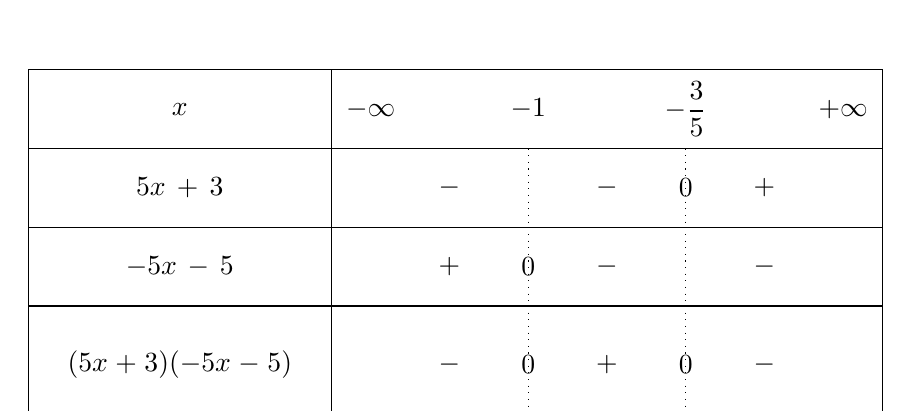
\begin{tikzpicture}
\tkzTabInit[lgt=3.85,espcl=2]{$x$ / 1, $5 x + 3$ / 1, $- 5 x - 5$ / 1, $(5 x + 3)(- 5 x - 5)$ / 1.5}{$-\infty$, $-1$, $- \dfrac{3}{5}$, $+\infty$}
\tkzTabLine{, -, t, -, z, +}
\tkzTabLine{, +, z, -, t, -}
\tkzTabLine{, -, z, +, z, -}
\end{tikzpicture}
\end{center}
\par\smallskip
\begin{center}$S = \left] -\infty \,;\, -1 \right] \cup \left[ - \dfrac{3}{5} \,;\, +\infty \right[$\end{center}\par\medskip
\noindent\textbf{2)}\par\smallskip
\begin{center}
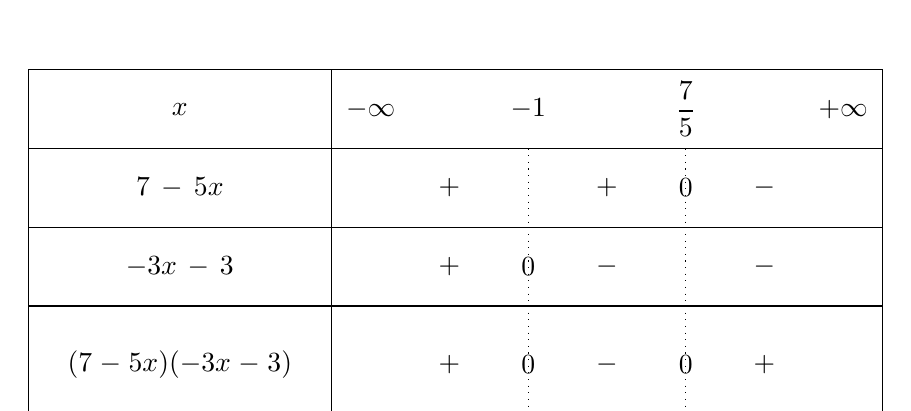
\begin{tikzpicture}
\tkzTabInit[lgt=3.85,espcl=2]{$x$ / 1, $7 - 5 x$ / 1, $- 3 x - 3$ / 1, $(7 - 5 x)(- 3 x - 3)$ / 1.5}{$-\infty$, $-1$, $\dfrac{7}{5}$, $+\infty$}
\tkzTabLine{, +, t, +, z, -}
\tkzTabLine{, +, z, -, t, -}
\tkzTabLine{, +, z, -, z, +}
\end{tikzpicture}
\end{center}
\par\smallskip
\begin{center}$S = \left] -1 \,;\, \dfrac{7}{5} \right[$\end{center}\par\medskip
\noindent\textbf{3)}\par\smallskip
\begin{center}
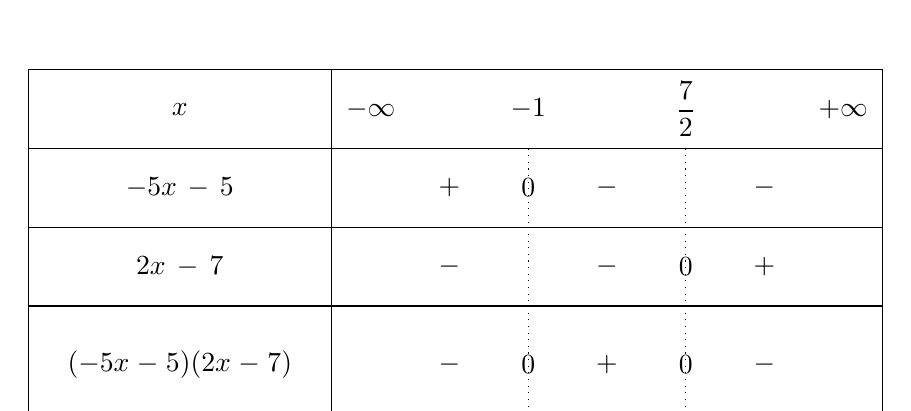
\begin{tikzpicture}
\tkzTabInit[lgt=3.85,espcl=2]{$x$ / 1, $- 5 x - 5$ / 1, $2 x - 7$ / 1, $(- 5 x - 5)(2 x - 7)$ / 1.5}{$-\infty$, $-1$, $\dfrac{7}{2}$, $+\infty$}
\tkzTabLine{, +, z, -, t, -}
\tkzTabLine{, -, t, -, z, +}
\tkzTabLine{, -, z, +, z, -}
\end{tikzpicture}
\end{center}
\par\smallskip
\begin{center}$S = \left] -\infty \,;\, -1 \right] \cup \left[ \dfrac{7}{2} \,;\, +\infty \right[$\end{center}\par\medskip
\noindent\textbf{4)}\par\smallskip
\begin{center}
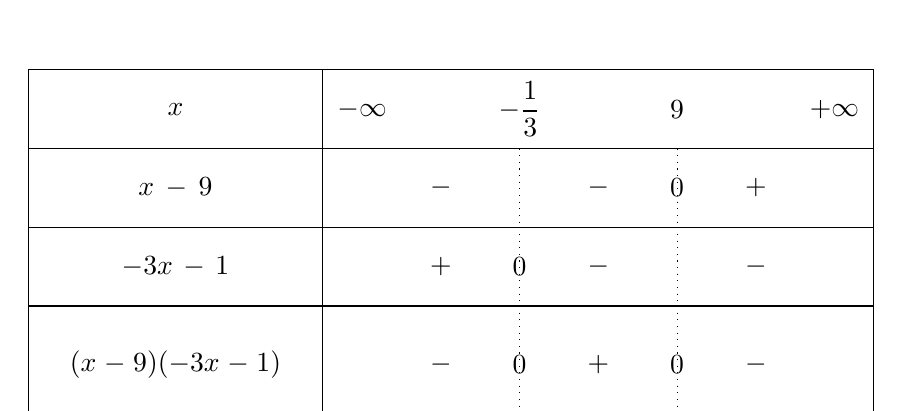
\begin{tikzpicture}
\tkzTabInit[lgt=3.74,espcl=2]{$x$ / 1, $x - 9$ / 1, $- 3 x - 1$ / 1, $(x - 9)(- 3 x - 1)$ / 1.5}{$-\infty$, $- \dfrac{1}{3}$, $9$, $+\infty$}
\tkzTabLine{, -, t, -, z, +}
\tkzTabLine{, +, z, -, t, -}
\tkzTabLine{, -, z, +, z, -}
\end{tikzpicture}
\end{center}
\par\smallskip
\begin{center}$S = \left] -\infty \,;\, - \dfrac{1}{3} \right] \cup \left[ 9 \,;\, +\infty \right[$\end{center}\par\medskip
\medskip

\noindent\textbf{Exercice 17}\par
\smallskip
\begin{enumerate}
\item $\dfrac{10^{-3} \times 10^{3}}{10^{3}} = 10^{-3}$
\item $\dfrac{10^{-2} \times (10^{3})^{3}}{10^{4}} = 10^{3}$
\item $\dfrac{10^{-2} \times 10^{0}}{10^{4}} = 10^{-6}$
\item $\dfrac{10^{-1} \times (10^{1})^{2}}{10^{4}} = 10^{-3}$
\end{enumerate}
\medskip

\noindent\textbf{Exercice 18}\par
\smallskip
\begin{enumerate}
\item $35 \sqrt{7}$
\item $49 \sqrt{5}$
\item $4 \sqrt{2}$
\item $- 3 \sqrt{5} + 7 \sqrt{13}$
\item $- 34 \sqrt{5}$
\item $16 - 8 \sqrt{3}$
\end{enumerate}
\medskip

\noindent\textbf{Exercice 19}\par
\smallskip
\textbf{1)}
\begin{enumerate}
\item $\overrightarrow{\ensuremath{\mathrm{A}}\ensuremath{\mathrm{B}}}(-7\,;\,-4)$
\item $\overrightarrow{\ensuremath{\mathrm{A}}\ensuremath{\mathrm{B}}}(3\,;\,-3)$
\item $\overrightarrow{\ensuremath{\mathrm{A}}\ensuremath{\mathrm{B}}}(0\,;\,2)$
\end{enumerate}
\textbf{2)}
\begin{enumerate}
\item $\ensuremath{\mathrm{M}}\left(-1\,;\,-7\right)$
\item $\ensuremath{\mathrm{M}}\left(-1\,;\,1\right)$
\end{enumerate}
\textbf{3)}
\begin{enumerate}
\item $\det(\vec{u},\vec{v}) = 1\times(6)-(3)\times2 = 0$. Oui.
\item $\det(\vec{u},\vec{v}) = -2\times(-4)-(-2)\times-5 = -2$. Non.
\end{enumerate}
\medskip

\noindent\textbf{Exercice 20}\par
\smallskip
\textbf{1)}
\begin{enumerate}
\item $m = \dfrac{-2--5}{0--4} = \dfrac{3}{4}$ donc $y = \dfrac{3}{4}x - 2$
\item $m = \dfrac{2-4}{0-3} = \dfrac{2}{3}$ donc $y = \dfrac{2}{3}x + 2$
\item $m = \dfrac{2-1}{4-1} = \dfrac{1}{3}$ donc $y = \dfrac{1}{3}x + \dfrac{2}{3}$
\end{enumerate}
\textbf{2)}
\begin{enumerate}
\item On cherche les couples $(x\,;\,y)$ vérifiant les deux équations :

$5x + 3 = -3x - 3$

$\Leftrightarrow 8x = -6$

$\Leftrightarrow x = - \dfrac{3}{4}$

puis $y = 5 \times (- \dfrac{3}{4}) + 3 = - \dfrac{3}{4}$

Donc le point d'intersection est $\left(- \dfrac{3}{4}\,;\,- \dfrac{3}{4}\right)$.
\item On cherche les couples $(x\,;\,y)$ vérifiant les deux équations :

$-x - 5 = 5x + 4$

$\Leftrightarrow -6x = 9$

$\Leftrightarrow x = - \dfrac{3}{2}$

puis $y = -(- \dfrac{3}{2}) - 5 = - \dfrac{7}{2}$

Donc le point d'intersection est $\left(- \dfrac{3}{2}\,;\,- \dfrac{7}{2}\right)$.
\end{enumerate}
\medskip

\newpage
\end{document}
